\documentclass[11pt]{report}
\usepackage{geometry}
\usepackage[utf8]{inputenc}
\usepackage[english,italian]{babel}
\usepackage{graphicx}
\usepackage{hyperref}
\usepackage{verbatim}
\usepackage{mathtools}
\usepackage{booktabs}
\usepackage{comment}
\usepackage{array}
\usepackage{caption}
\usepackage{subcaption}
\usepackage{capt-of}
\usepackage{rotating}
\usepackage{floatpag}
\usepackage{pdflscape}
\usepackage[toc,page]{appendix}

\newcommand\frontmatter{%
    \cleardoublepage
  %\@mainmatterfalse
  \pagenumbering{Roman}}

\newcommand\mainmatter{%
    \cleardoublepage
 % \@mainmattertrue
  \pagenumbering{arabic}}

\newcommand\backmatter{%
  \if@openright
    \cleardoublepage
  \else
    \clearpage
  \fi
 % \@mainmatterfalse
   }




\geometry{a4paper, top=4cm, bottom=4cm, left=3.7cm, right=3.7cm}


\usepackage{listings}
\usepackage{xcolor}

%New colors defined below
\definecolor{codegreen}{rgb}{0,0.6,0}
\definecolor{codegray}{rgb}{0.5,0.5,0.5}
\definecolor{codepurple}{rgb}{0.58,0,0.82}
\definecolor{backcolour}{rgb}{0.95,0.95,0.92}

%Code listing style named "mystyle"
\lstdefinestyle{mystyle}{
  backgroundcolor=\color{backcolour},   commentstyle=\color{codegreen},
  keywordstyle=\color{magenta},
  numberstyle=\tiny\color{codegray},
  stringstyle=\color{codepurple},
  basicstyle=\ttfamily\footnotesize,
  breakatwhitespace=false,         
  breaklines=true,                 
  captionpos=b,                    
  keepspaces=true,                 
  numbers=left,                    
  numbersep=5pt,                  
  showspaces=false,                
  showstringspaces=false,
  showtabs=false,                  
  tabsize=2
}

%"mystyle" code listing set
\lstset{style=mystyle}



\begin{document}

\frontmatter

\title{Bozza Tesi Magistrale}

\author{Mattia Marchi 817587 }

\date{}

\maketitle



\newpage

\begin{abstract}
In questo progetto di tesi viene presentato un nuovo approccio per la creazione di un sistema di raccomandazione e generazione di playlist, utilizzando modelli di Deep Learning per riconoscere le emozioni degli utenti associate alla musica. L'ambito di ricerca è definito\textit{ Music Emotion Recognition }(MER), sottocategoria dell’\textit{Affective Computing}, branca dell’intelligenza artificiale che riconosce ed utilizza le emozioni umane. Al giorno d'oggi i sistemi MER stanno avendo sempre più risalto, grazie all'integrazione con sistemi di raccomandazione, a fronte della vasta popolarità delle piattaforme streaming di riproduzione musicale. 

Il modello proposto è composto da diverse tipologie di reti neurali profonde. Inizialmente si utilizza una rete neurale convoluzionale (CNN), facendo uso della tecnica definita \textit{transfer learning} su un’architettura allo stato dell'arte per estrarre le informazioni più rilevanti da spettrogrammi di Mel, quest’ultimi generati da file musicali. Successivamente si impiega una rete Long Short-Term Memory (LSTM) per classificare correttamente le feature estratte. Le classi emozionali esaminate corrispondono ai quattro quadranti del modello di Russell. I dataset, impiegati nella realizzazione del modello di Deep Learning, sono stati selezionati dalla letteratura di riferimento al fine di considerare multiple fonti per migliorare la generalizzazione. Il risultato di accuratezza raggiunto dal modello finale è pari al 91\%. 


È stata inoltre studiata la capacità del modello finale di adattarsi alla percezione del singolo individuo, tramite la tecnica di \textit{fine-tuning} sulle emozioni soggettive di ogni utente. Questo secondo modello prende il nome di "user-tuned". L'obiettivo principale è quello di ottenere un sistema inizialmente capace di generalizzare, minimizzando l'errore nell’uso da parte di nuovi utenti, e successivamente adattarlo al singolo utente e alle sue percezioni soggettive. Tale metodologia consente di accentuare il focus sul singolo soggetto, migliorando l'esperienza di utilizzo e risolvendo uno dei problemi principali dei sistemi di raccomandazione: il \textit{cold start}. Il sistema è stato testato su tre soggetti, utilizzando 50 canzoni di diverso genere, mostrando un'accuratezza nel predire correttamente le emozioni del 44.68\% per il modello generale. Il test effettuato sul modello user-tuned, considerando 10 e 20 emozioni suggerite al sistema, ha raggiungo un valore medio di predizioni corrette del 62.66\% e 76\% rispettivamente, migliorando fortemente i risultati ottenuti dal modello generale. I risultati empirici hanno inoltre dimostrato che il modello user-tuned riesce a perfezionare le inferenze delle canzoni non suggerite direttamente al sistema, abbassando l'errore di predizione medio. 


Infine, è stato creato un sistema di raccomandazione, il quale utilizza le informazioni ottenute dai modelli precedentemente descritti per generare una playlist personalizzata in base all'umore attuale dell'utente ed uno stato emozionale target da raggiungere. La generazione viene effettuata in modo tale da creare un graduale passaggio emozionale, utilizzando canzoni proprie e migliorando l'esperienza finale dell'utente.



\end{abstract}




\newpage

\tableofcontents

\listoffigures

\listoftables


\newpage

\mainmatter

\chapter{Introduzione}

Negli ultimi decenni si è assistito ad un'esplosione della quantità di dati digitali condivisi nel web. Gli utenti avvertono sempre più la necessità di sistemi che possano filtrare in modo automatizzato i contenuti, così che gli vengano proposti solo quelli di loro potenziale interesse. Con questo obiettivo, nei primi anni '90 sono stati sviluppati i primi \textit{Recommender System} (RS) che hanno rivoluzionato l'e-commerce e la fruizione di contenuti da parte delle persone \cite{Konstan2012Apr}. Dal momento della loro nascita fino ai giorni d'oggi, sono stati diversi gli sviluppi ed i contesti in cui tali sistemi hanno operato e continuano tuttora a farlo. Uno di questi campi è quello musicale. 
Oggigiorno, le persone trascorrono ore intere ad ascoltare la propria musica preferita. Il rapporto sulle abitudini del consumo musicale, realizzato dall'IFPI, relativo all'anno 2021 ha rivelato che il tempo a cui le persone di tutto il mondo dedicano all'ascolto della musica è in continuo aumento. Secondo \emph{International Federation of the Phonographic Industry}, a livello globale si è raggiunta una media di ascolto settimanale pari a 18.4 ore, mentre localizzando l'analisi solamente all'Italia questo dato cresce fino a 19.1 ore \cite{BibEntry2022Feb}. Differenti studi hanno mostrato come l'ascolto della musica abbia un impatto decisivo sul cambiamento delle emozioni che le persone provano nel breve periodo e sulla loro capacità di affrontare situazioni difficili. Per esempio, Lehmberg \textit{et al.}\cite{Lehmberg2010BenefitsOM} hanno scoperto evidenza di diversi benefici che la musica dal vivo può portare alle persone anziane: potenziale incremento dell'aspettativa di vita, minore stress, miglioramento della situazione medica e complessivo aumento della felicità. Secondo uno studio congiunto dell'università di Durham in Inghilterra e dell'università di Jyväskylä in Finlandia \cite{Eerola2016Jun} anche la musica più triste può portare alle persone conforto e appagamento. Nonostante ciò, lo stesso studio ha anche evidenziato come questo tipo di musica possa causare in alcuni soggetti sofferenza. 
Un'ulteriore studio del 2013 \cite{Ferguson2013Jan} ha portato evidenza del fatto che l'ascolto della musica allegra può portare ad un miglioramento complessivo dell'umore delle persone in sole due settimane.\\

\newpage

Diverse ricerche nell'ambito della psicologia, applicata al contesto musicale, hanno confermato che la musica può indurre nell'ascoltatore una risposta emozionale molto forte \cite{Krumhansl}\cite{Mitterschiffthaler2007Nov}\cite{Charlotte}. Le emozioni e i sentimenti hanno suscitato fin dai tempi più antichi interesse ed attenzione da parte di filosofi, psicologi, dottori e ricercatori che lavorano in questi ambiti \cite{Barrett2006Mar}. Lo studio delle emozioni è nato svariati secoli fa e con il passare degli anni ne sono state fornite molteplici definizioni. Gran parte delle teorie moderne definiscono le emozioni come un processo multicomponenziale, ovvero formato da distinte componenti in continua evoluzione nel corso del tempo. Alcuni studiosi descrivono le emozioni come forti sensazioni che nascono in seguito al verificarsi di esperienze, positive o negative \cite{knuuttila2004emotions}. Altri ricercatori invece, le caratterizzano come stati psicologici provocati da cambiamenti neuro-fisici associati a pensieri, sentimenti e risposte comportamentali \cite{Chaturvedi2022Feb}.


Negli ultimi anni è nato un crescente interesse relativo allo sviluppo di sistemi che integrano le emozioni, al fine di garantire all'utente un'esperienza personalizzata più gratificante. La branca dell'intelligenza artificiale che studia il riconoscimento e l'utilizzo delle emozioni viene chiamata Affective Computing\cite{picard2000affective}. La nascita di tali tecniche, integrate in applicazioni musicali, ha portato allo sviluppo di sistemi di riconoscimento delle emozioni e di generazione di playlist basate sul mood attuale dell'utente.

\section{Obiettivi della Tesi}



In questo lavoro viene esplorata la possibilità di creare un sistema di raccomandazione e generazione di playlist basato sull'unione di diversi modelli di Deep Learning. L'idea alla base del progetto è quella di sfruttare alcuni dei dataset più completi presenti nella letteratura di riferimento, nell'ambito del riconoscimento emozionale applicato alla musica, al fine di progettare un modello efficace nell'effettuare predizioni emozionali, basandosi solo sulle feature audio delle canzoni. La scelta dei modelli di Deep Learning - chiamati reti neurali profonde - è stata effettuata in base alla capacità delle reti di sfruttare grandi quantità di dati per creare sistemi capaci di riconoscere pattern e feature rilevanti, ed utilizzare tali informazioni in modo tale da effettuare task predittivi o di regressione.


Il sistema in questione sarà in grado di classificare ed etichettare le canzoni dell'utente che lo utilizzerà, sulla base delle diverse emozioni che l'ascolto può indurre nel soggetto, riconosciute dalla rete neurale. L'architettura è progettata per essere applicata ad immagini generate dai file audio, chiamati spettrogrammi di Mel. La classificazione si baserà su due diversi modelli, studiati per essere utilizzati in diverse casistiche reali. Il primo - chiamato modello generale - sarà formato da un insieme di reti neurali, capaci di stimare che tipo di umore può evocare l'ascolto di una canzone per la maggior parte degli utenti, minimizzando il rischio di errore nella predizione. Questo aspetto risulta fondamentale per far sì che anche nuovi utenti, approcciandosi al sistema per la prima volta, riescano a trovarsi d'accordo con l'emozione proposta. Il secondo modello - chiamato "user-tuned" - sarà invece un adattamento di quello generale in grado di imparare dal singolo utente, durante l'utilizzo del sistema, addestrando la rete a considerare la sua percezione soggettiva. Tale considerazione risulta di vitale importanza in un lavoro di affective computing, proprio perché le emozioni indotte dalla musica e la loro percezione sono esperienze estremamente soggettive e dunque risulta significativo considerare tale aspetto. La tecnica usata per adattare il modello generale all'utente, creando quello che è stato definito user-tuned, è chiamata fine-tuning. Tale tecnica consentirà ad ogni utente di definire molteplici nuovi esempi al modello, basati sulla propria percezione, così da addestrarlo alla soggettività emotiva del soggetto, andando quindi ad affinare ulteriormente il sistema di raccomandazione. Il sistema, come obiettivo finale, dovrà generare automaticamente delle playlist, basate sull'umore attuale dell'utente ed utilizzando canzoni in suo possesso, consentendo a quest'ultimo di definire uno stato emozionale target da raggiungere alla fine dell'ascolto.\\


% Tale classificazione non solo potrà essere effettuata da un utente che si approccia al sistema per la prima volta, attraverso un modello studiato per essere abile nella generalizzazione, ma si potrà inoltre adattare il modello all'utente stesso, sfruttando una tecnica chiamata fine-tuning.

\section{Outline}

Questo documento è composto da 8 capitoli, di cui segue una breve descrizione:

\begin{itemize}

    \item Questo capitolo introduce l'ambito di studio della tesi, il progetto preso in esame e ne descrive brevemente la struttura;
    
    \item Il secondo capitolo richiama alcune nozioni teoriche necessarie alla comprensione del testo;
    
    \item Il terzo capitolo descrive i principali approcci esistenti, applicati al problema di riconoscimento emozionale musicale, descritti in letteratura;

    \item Il quarto capitolo descrive i dataset di riferimento utilizzati nello sviluppo dei modelli impiegati nel progetto. Viene inoltre esposta la fase di preprocessing dei dati;
    
    \item Il quinto capitolo descrive i modelli di deep learning progettati, fornendo alcuni dettagli tecnici di realizzazione ed analizzando i risultati ottenuti;
    
    \item il sesto capitolo pone il focus sul processo definito di user-tuning, descrivendone la metodologia e mostrandone il funzionamento ed i risultati empirici ottenuti;
    
    \item Il settimo capitolo chiude la descrizione del progetto descrivendo come i modelli ideati vengano utilizzati dal sistema di raccomandazione e generazione di playlist;
    
    \item L'ultimo capitolo conclude la tesi andando a riassumere i risultati ottenuti ed i possibili sviluppi futuri.
\end{itemize}

\chapter{Quadro Teorico}

In questo capitolo vi è un'introduzione di tutti i concetti fondamentali necessari a comprendere ciò che verrà trattato in questo lavoro.


\section{Deep Learning}

Il Deep Learning (DL) rappresenta una branca dell'intelligenza artificiale che studia modelli, basati su reti neurali, che contengono molteplici strati nascosti, creando una struttura definita "profonda". Tali reti si utilizzano per effettuare processi di apprendimento automatico, chiamato anche Machine Learning (ML), imparando feature rilevanti relative ad uno o più dataset, osservando una grande quantità di esempi forniti dai dati. Ai fini della tesi verranno presentate le due principali tipologie di reti implementate nel progetto: Convolutional Neural Network (CNN) e Long Short-Term Memory (LSTM).


\subsection{Convolutional Neural Networks}
Una Convolutional Neural Network rappresenta un'architettura di rete neurale profonda ideata per classificare immagini \cite{krizhevsky2012imagenet}. Tale architettura, ispirata alla biologia, consente di osservare porzioni locali di un'immagine, utilizzando dei filtri per imparare diverse \textit{feature map}. Attraverso questo sistema la rete è capace di capire le relazioni tra i pixel ed a estrarre feature spaziali locali. Ogni strato convoluzionale è formato da dimensioni (altezza, larghezza, canali cromatici) ed un numero di filtri. Gli strati convoluzionali sono seguiti da una funzione di attivazione e un layer di pooling spaziale, usato per ridurre la dimensione dell'input. Negli anni, grazie alla ricerca e per merito di diversi contest come \textit{ImageNet}, le reti convoluzionali hanno subito vasti miglioramenti alle performance, sviluppando reti sempre più complesse. Al fine di addestrare una CNN in un task di classificazione, viene aggiunta in coda una rete neurale Fully-Connected (FC) che, grazie alle feature ottenute dalla CNN, effettuerà la predizione.  È possibile osservare quanto descritto in figura \ref{fig:cnn}



\begin{figure}[h]
    %\hspace{-1cm}
    \centering
    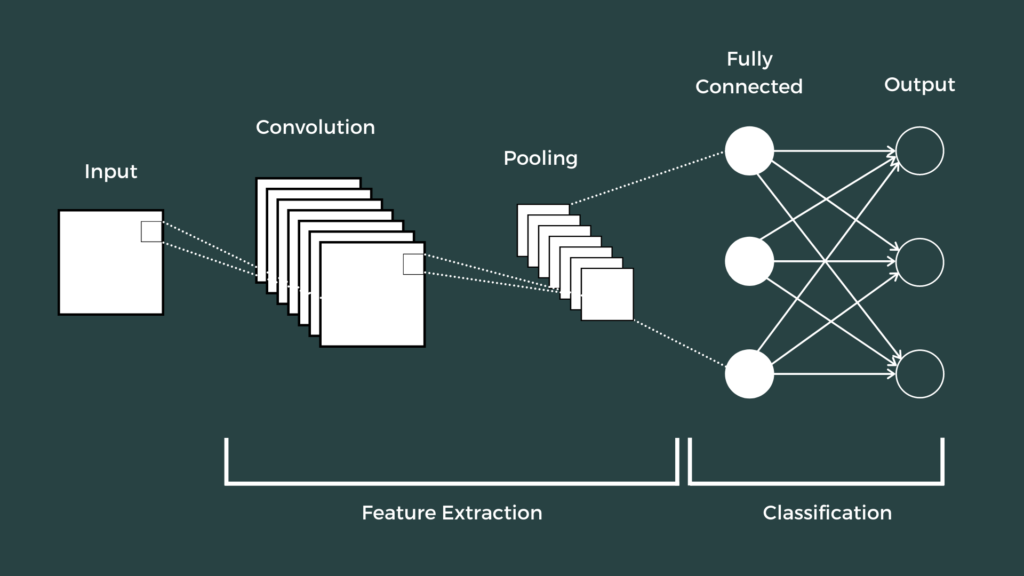
\includegraphics[scale = 0.3]{img/cnn.png}
    \caption[Struttura di una rete neurale convoluzionale.]{Struttura di una rete neurale convoluzionale.\footnotemark}
    \label{fig:cnn}
\end{figure}


\footnotetext{Source: \url{https://www.theclickreader.com/building-a-convolutional-neural-network/}}


Per addestrare una rete CNN è necessario avere un dataset abbastanza numeroso ed una grande potenza di calcolo, pertanto è raro che si utilizzi una rete creata ad hoc. La scelta più popolare è quella di utilizzare il processo chiamato \textit{tansfer learning}. Questa metodologia consente di usufruire di reti pre-addestrate e adattarle al task del dominio specifico. Esistono due diversi tipi di transfer learning:
\begin{itemize}
    \item \textbf{Fine-Tuning}: i pesi vengono mantenuti bloccati o viene utilizzato un learning rate molto basso per non variare troppo i pesi originali. La rete fully connected finale viene invece sostituita per ottenere una nuova rappresentazione, così da poterla addestrare mantenendo i pesi della CNN. 
    

    \item \textbf{Feature Extractor}: si taglia la rete all'ultimo layer convoluzionale e si ottiene un vettore di feature, chiamato \textit{descriptor}, il quale verrà utilizzato in un nuovo classificatore.

\end{itemize}

\subsection{Long Short-Term Memory}

La famiglia di reti neurali specializzate nel processare dati sequenziali è chiamata Recurrent Neural Network (RNN) \cite{rumelhart1985learning}. Queste reti vengono chiamate ricorrenti perché elaborano i dati come sequenze ed ogni output dipende dalla computazione dello stato precedente. La sotto-classe delle RNN più utilizzata al giorno d'oggi è quella chiamata Long Short-Term Memory (LSTM)\cite{hochreiter1997long}. Tale rete è formata da diversi stati interni e \textit{gate}, i quali permettono di controllare il flusso delle informazioni. I gate inoltre consentono al modello di dimenticarsi delle informazioni di poco rilievo, mantenendo solo quelle rilevanti. Nel dettaglio, una rete LSTM è composta dai seguenti componenti:
\begin{itemize}
    \item \textbf{Cell State}: prende in input l'output della sequenza precedente e, in base ai gate, mantiene o cancella tale informazione;
    
    \item \textbf{Forget Gate}: utilizza una funzione sigmoide, prende in input la concatenazione dell'output della sequenza precedente e l'input della sequenza attuale, determinando se l'informazione vecchia debba essere mantenuta o cancellata;
    
    \item \textbf{Input Gate}: determina se l'input della sequenza attuale verrà aggiunto al cell state;
    
    \item \textbf{Output Gate}: lo stato finale del cell state viene filtrato da una funzione tangente ($-1,1$), determinando il nuovo output.
    
\end{itemize}
La struttura di una rete LSTM è mostrata in figura \ref{fig:lstm}.


\begin{figure}[h]
    %\hspace{-1cm}
    \centering
    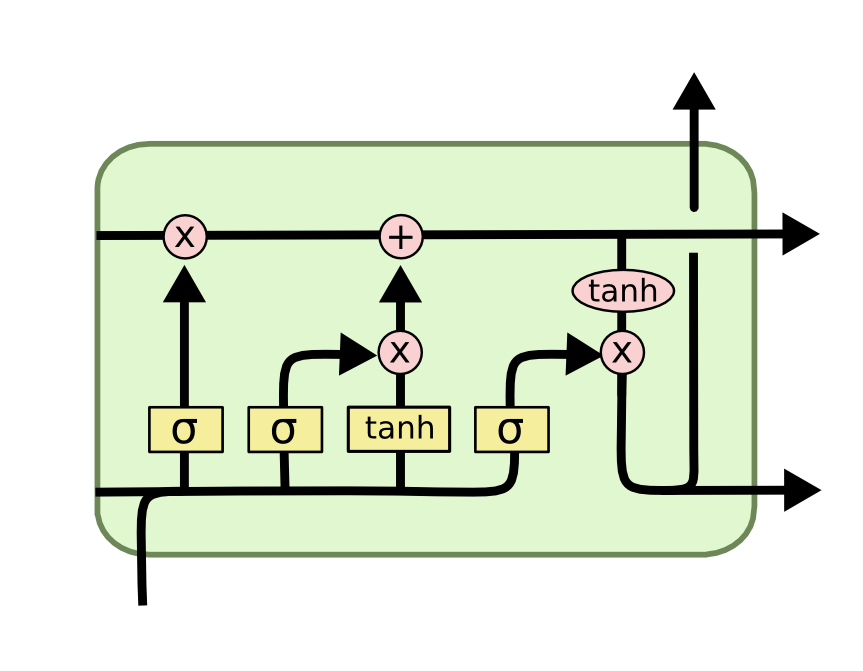
\includegraphics[scale = 0.7]{img/lstm.png}
    \caption[Struttura a gate di una rete LSTM.]{Struttura a gate di una rete LSTM.\footnotemark}
    \label{fig:lstm}
\end{figure}


\footnotetext{Source: \url{https://colah.github.io/posts/2015-08-Understanding-LSTMs/}}



\section{Le Emozioni}


Diversi ricercatori e psicologi hanno definito alcuni modelli per classificare le emozioni, fondati su diverse teorie. Tuttavia, in letteratura esistono principalmente due famiglie di approcci con cui è possibile descrivere lo stato emotivo di una persona. Il primo di questi prevede di suddividere le emozioni in uno spazio discreto, formando alcuni gruppi di aggettivi, i quali rappresentano ciascuno un'emozione. Tale modello assume l'esistenza di un insieme limitato di categorie emozionali distinte. Uno dei modelli più rilevanti che appartiene a questa categoria è quello descritto da Plutchik \cite{plutchik2013theories}, che divide le emozioni in 8 categorie rappresentate mediante la cosiddetta "\textit{wheel of emotions}", mostrata in figura \ref{fig:wheel}. L'intensità delle emozioni cresce dall'esterno verso il centro della ruota. Più è scuro il colore, maggiore è l'intensità dell'emozione.

\begin{figure}[h]
    %\hspace{-1cm}
    \centering
    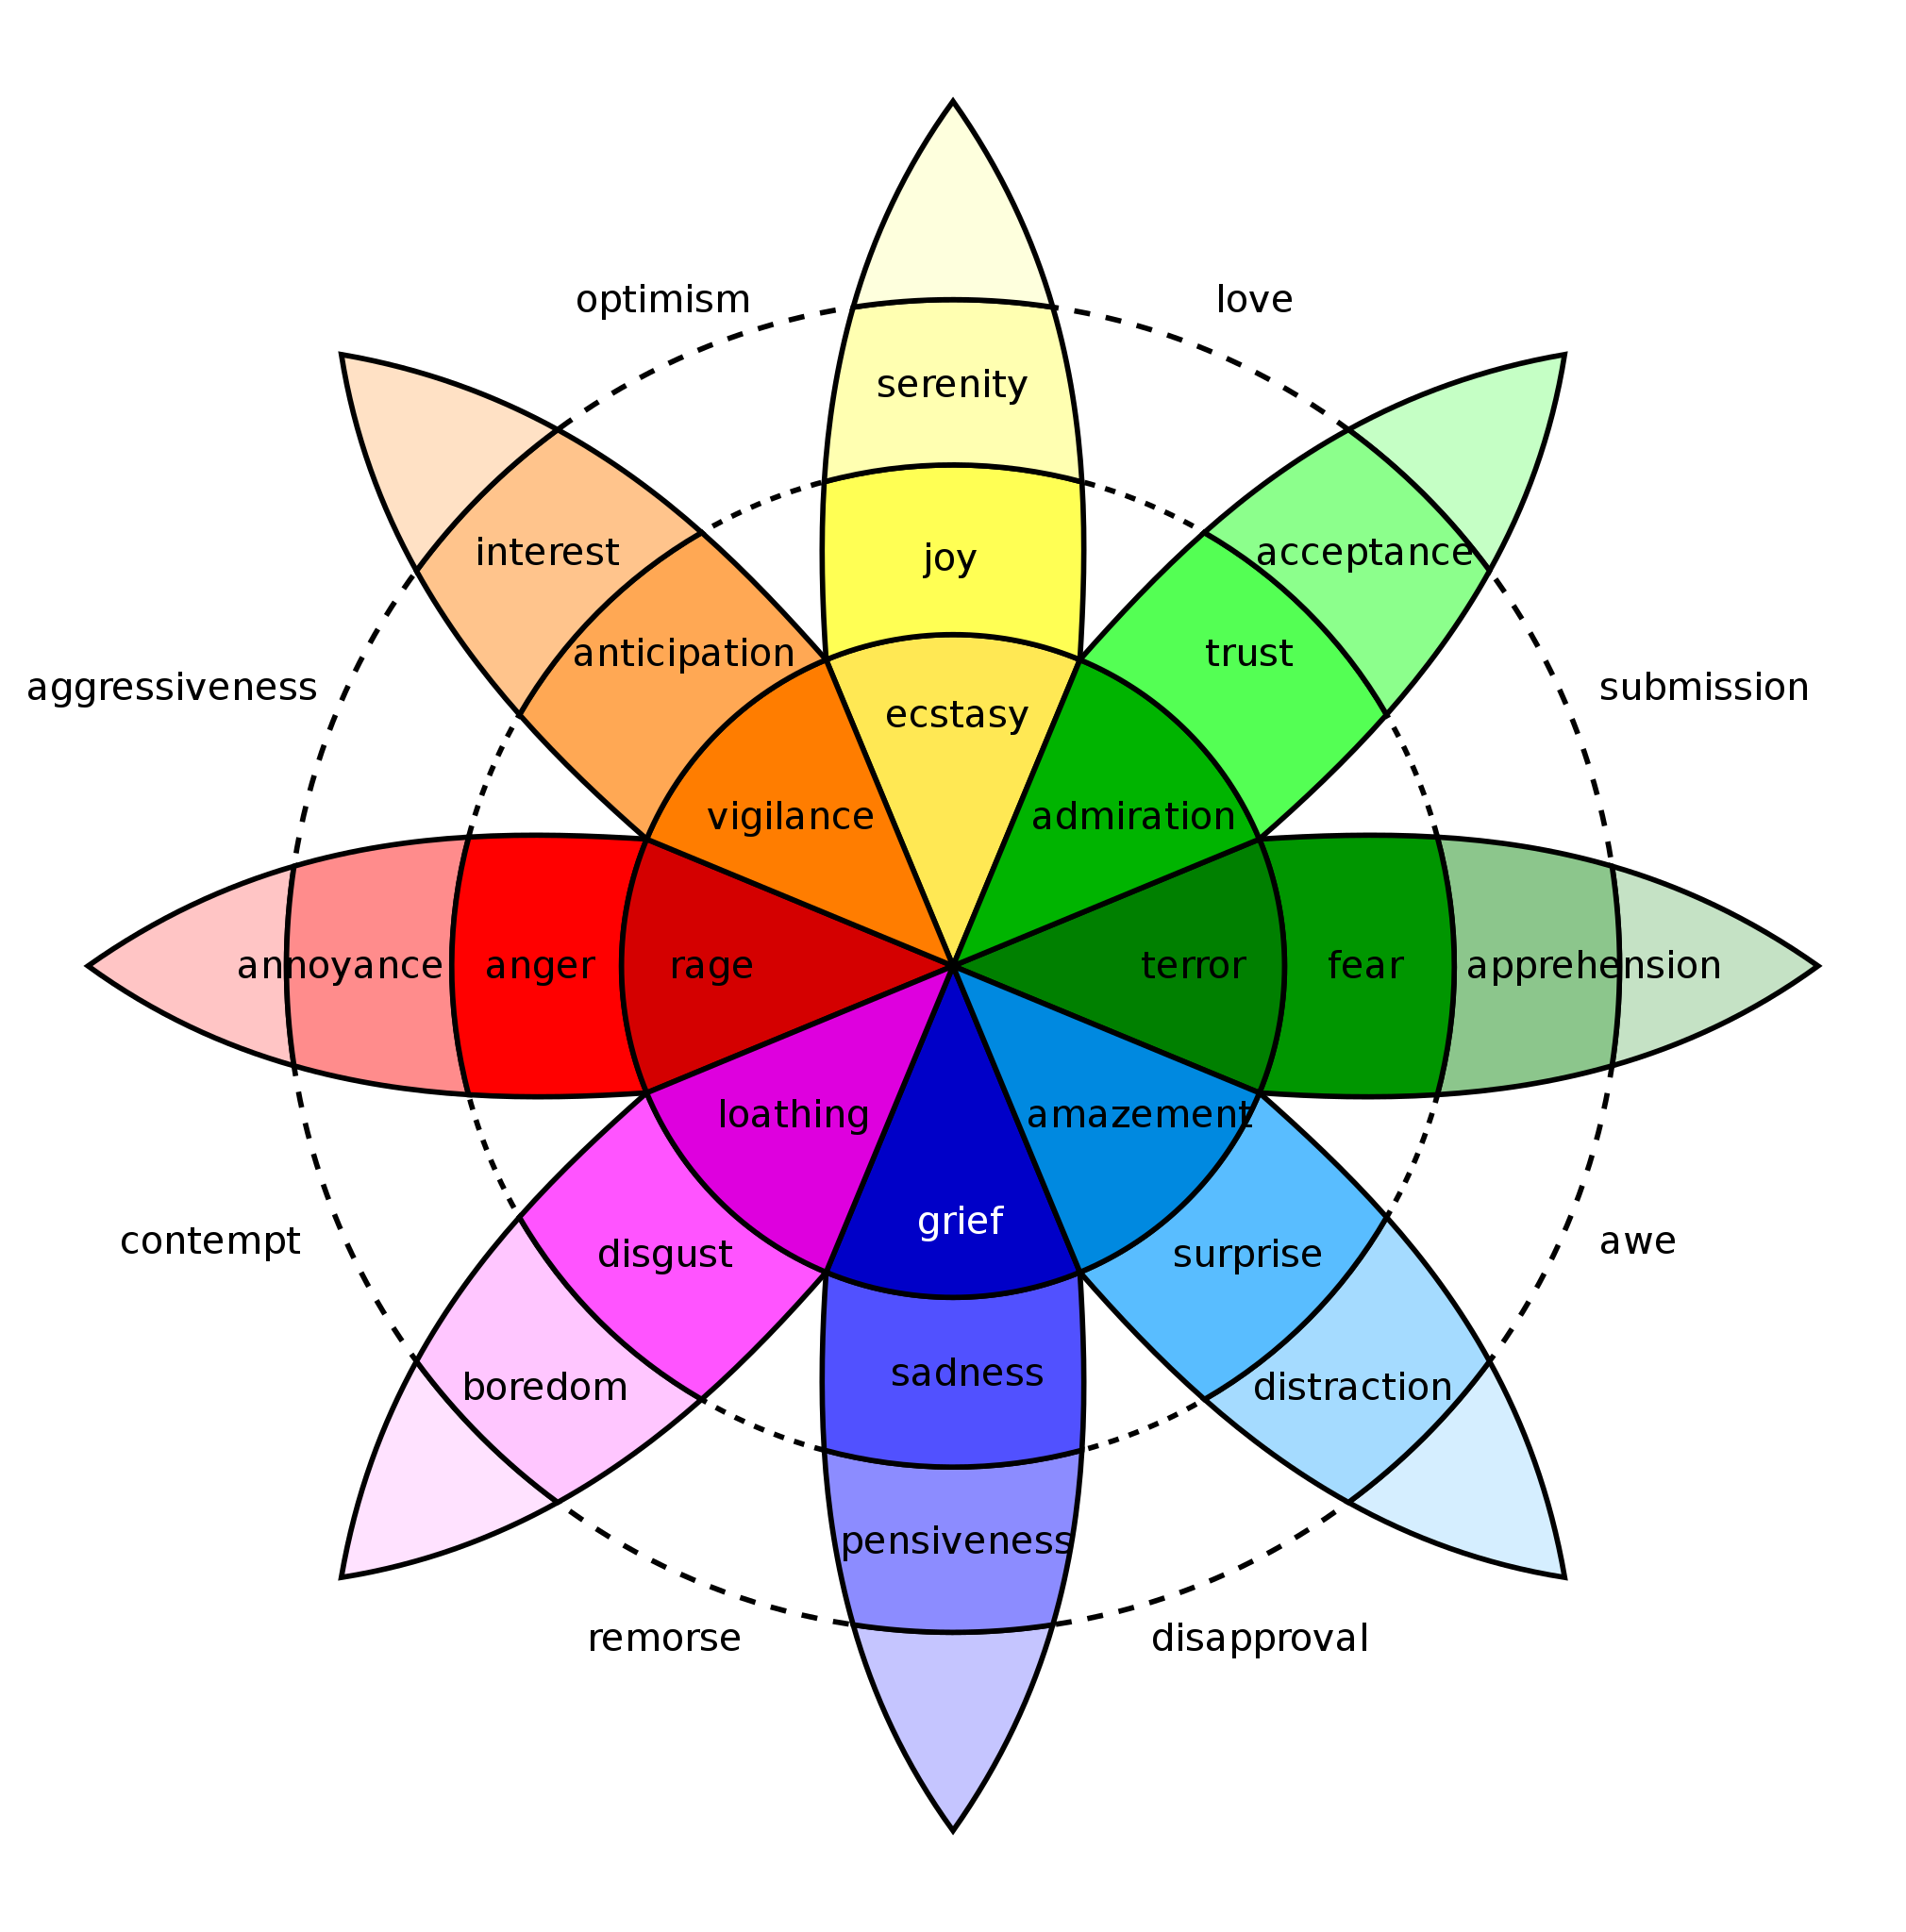
\includegraphics[scale = 0.15]{img/Plutchik-wheel.svg.png}
    \caption[\textit{Wheel of emotions} proposta da Plutchik.]{\textit{Wheel of emotions} proposta da Plutchik.\footnotemark}
    \label{fig:wheel}
\end{figure}

\footnotetext{Source: \url{https://commons.wikimedia.org/wiki/File:Plutchik-wheel.svg}}

\newpage

La seconda famiglia di modelli segue un approccio dimensionale. Tale approccio descrive ogni emozione come un punto in uno spazio continuo ed ogni dimensione rappresenta una aggettivo che caratterizza l'emozione stessa. Il modello più frequentemente utilizzato appartenente a questa categoria è quello proposto da James Russell \cite{Russel}, chiamato \textit{Circumplex Model}. Russell suggerisce che le emozioni siano distribuite in uno spazio circolare bidimensionale, il quale è composto da due dimensioni: attivazione - definito come \textit{arousal} o \textit{activation} - che indica l'intensità dell'emozione percepita e la valenza - o \textit{valence} - che esprime la polarità dell'emozione come positiva o negativa. L'arousal rappresenta l'asse verticale, mentre la valence rappresenta l'asse orizzontale. Ogni stato emozionale può essere rappresentato come un punto in questo spazio bidimensionale. Questa classificazione ha il vantaggio, tramite l'utilizzo di uno spazio continuo, di poter utilizzare valori compresi tra $[0,1]$ per esprimere ogni possibile tipologia di emozione come una coordinata sul piano. È inoltre possibile inserire emozioni categoriche in questo spazio bidimensionale, così da poter effettuare una conversione tra i due modelli descritti. Una rappresentazione del modello proposto da Russell è visibile in figura \ref{fig:russell}.

\newpage

\begin{figure}[h]
    %\hspace{-1cm}
    \centering
    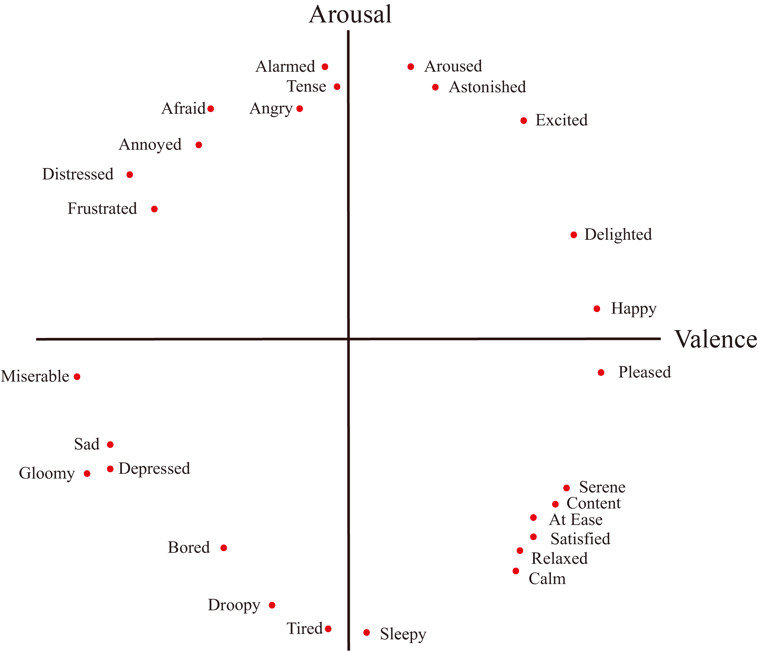
\includegraphics[scale = 0.38]{img/Russells-circumplex.jpg}
    \caption{Il quadrante delle emozioni proposto da Russell. \cite{seo2019automatic}}
    \label{fig:russell}
\end{figure}



\section{Sistemi di Raccomandazione}


Nell'ambito dell'intelligenza artificiale, con sistema di raccomandazione - o \textit{recommender system} - si intende una classe di algoritmi di machine learning usati dagli sviluppatori software per effettuare predizioni sulle scelte dell'utente ed offrire ad esso consigli rilevanti \cite{indatalabs}.  
Esistono principalmente quattro tipologie di recommender system: \textit{collaborative filtering}, \textit{content based filtering}, \textit{demographic filtering} ed i sistemi \textit{ibridi} \cite{re-sys-survey}. Il primo di questi approcci ricerca similarità e relazioni tra gli utenti che usano il sistema. In particolare, questi modelli consigliano ad un utente \emph{$\alpha$} i contenuti che sono stati apprezzati da un utente \emph{$\beta$} simile ad \emph{$\alpha$} stesso. Viceversa, i modelli appartenenti alla seconda categoria effettuano delle raccomandazioni esclusivamente analizzando le feature e le descrizioni degli oggetti che sono stati valutati positivamente dagli utenti, al fine di consigliagliene altri simili. I modelli demografici invece sfruttano il principio per cui individui con attributi simili (ad esempio sesso, età, paese di provenienza ecc.) avranno preferenze comuni. Infine, l'approccio ibrido prevede di combinare le tecniche utilizzate dagli altri approcci per ottenere risultati superiori.

Un ulteriore divisione nella tassonomia dei recommender system è data dal metodo con cui si effettua la raccomandazione. Esistono infatti due principali categorie: \textit{memory-based} e\textit{ model-based}\cite{re-sys-survey}. Il primo metodo utilizza lo storico delle valutazioni dell'utente sui prodotti per calcolare la distanza tra due diversi utenti o \textit{items}. Il metodo model-based invece utilizza modelli di machine learning per effettuare predizioni sulle preferenze dell'utente ed effettuare raccomandazioni. I modelli più utilizzati sono matrix factorization, classificatori Bayesiani, reti neurali, algoritmi genetici e logica fuzzy. Si utilizzano inoltre tecniche di dimensionality reduction, al fine di ridurre la sparsità dei dati.


Un problema noto dei sistemi di raccomandazione è chiamato \textit{cold start} \cite{re-sys-survey}. Tale evento si può verificare in vari modi e porta ad avere difficoltà nella raccomandazione. Un primo caso si verifica quando non si hanno abbastanza informazioni sull'utente, appena iscritto alla piattaforma utilizzante il recommender system, per effettuare raccomandazioni accurate. In questo caso si parla di \textit{new user problem}. Un secondo caso è quando un nuovo oggetto viene aggiunto al sistema: esso non avrà abbastanza recensioni per essere adeguatamente raccomandato al giusto cluster di utenti, prendendo il nome di \textit{new item problem}. La soluzione proposta in questa tesi è stata ideata con il fine di risolvere tali problemi, come si potrà riscontrare nei capitoli successivi.\\

\subsection{Sistemi di Raccomandazione in Ambito Musicale}

Il lavoro su cui si basa questa tesi riguarda un dominio specifico, ovvero quello musicale. È importante sottolineare questo aspetto poiché esistono sostanziali differenze rispetto ad altri sistemi di raccomandazione in differenti ambiti.
Batmaz \textit{et al.} \cite{deep-re-sys-survey} hanno effettuato uno studio comparativo dei diversi sistemi di raccomandazione, in dominio musicale, presenti in letteratura. Tale studio ha evidenziato le tipologie differenti di dati utilizzati e le ha classificate in tre diverse categorie: 
\begin{itemize}
    \item \textbf{Segnali Audio}: si utilizzano feature estratte dai segnali audio per addestrare il modello su cui si basa il sistema di raccomandazione;
    
    \item \textbf{Informazione Content-Based}: si utilizzano le informazioni relative agli utenti e/o items, utilizzando dataset eterogenei;
    
    \item \textbf{Valutazioni ed Utilizzo}: si utilizzano le informazioni relative all'ascolto musicale e le valutazioni per selezionare i brani da raccomandare.
\end{itemize}
In figura \ref{fig:musical-RS} è possibile osservare uno schema rappresentante la scelta delle feature utilizzate in 9 studi, presenti in letteratura, di recommender system in ambito musicale. Si osserva come quasi la totalità degli studi utilizzano le valutazioni e gli ascolti per effettuare la raccomandazione e solo in alcuni casi si associano questi dati ai segnali audio o alle informazioni content-based. Un limite di questi studi risulta essere quello di non considerare le emozioni nell'effettuare raccomandazioni agli utenti, ignorando i relativi vantaggi.

\vspace{1cm}

\begin{figure}[h!]
	 	\centering
	 	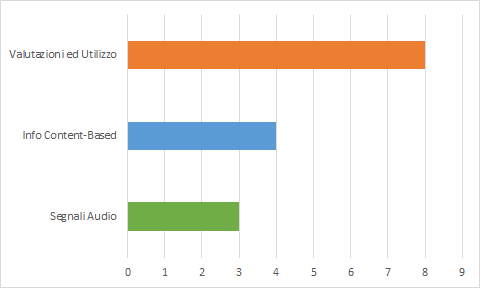
\includegraphics[scale = 0.95]{img/survery-RS.png}
	 	\caption{Distribuzione tipologie di dati utilizzati come feature su 9 studi riguardanti RS in ambito musicale.\cite{deep-re-sys-survey}}
	 	\label{fig:musical-RS}
\end{figure}


\chapter{Stato dell'Arte}

In questo capitolo vengono illustrate diverse tipologie di modelli presenti in letteratura nell'ambito di sistemi di riconoscimento delle emozioni. Al fine di utilizzare le emozioni in un sistema di raccomandazione musicale è necessario creare un modello capace di riconoscere i possibili stimoli emozionali suscitati nell'ascolto. I sistemi capaci di riconoscere emozioni in ambito musicale vengono definiti di \textit{Music Emotion Recognition} (MER). I sistemi MER sfruttano tecniche per elaborare diversi tipi di informazioni, al fine di riconoscere quale tipo di emozione sarà associata ad una canzone.


Kim \textit{et al.} \cite{kim2010music} hanno effettuato uno studio di diverse tipologie di approcci utilizzati nell'ambito dei sistemi MER, suddividendoli in due macro categorie: \textit{contextual text information} e \textit{content-based audio analysis}.

\section{Contextual Text Information}

In questi sistemi si utilizzano informazioni testuali per effettuare la predizione dell'emozione suscitata nell'utente. Le principali tecniche utilizzate in questo approccio sono tecniche di \textit{Information Retrieval} (IR), \textit{Text Mining} e \textit{Natural Language Processing} (NLP). Esistono diverse tipologie di sistemi che utilizzano tali informazioni:
\begin{itemize}
    \item \textbf{Riconoscimento emozionale dal testo}:
    questa tecnica utilizza il testo della canzone - o \textit{lyrics} - per riconoscere l'emozione che essa vuole trasmettere. Malheiro \textit{et al.} \cite{lyrics} hanno effettuato uno studio comparativo di questa metodologia rispetto alla controparte content-based. Per l'estrapolazione delle feature dal testo la metodologia risultata più promettente è stata la \textit{Bag-Of-Word} (BOW) \cite{sebastiani2002machine}. Tale tecnica, applicata al NLP, consente di creare una rappresentazione vettoriale del testo, composta dal numero di occorrenze delle parole, ed estrarre feature da esso. Il vantaggio di questa tecnica è quello di poter applicare modelli di machine learning sulle feature estratte. Tuttavia, i risultati ottenuti, applicando un classificatore \textit{Support Vector Machine} (SVM), hanno dimostrato sperimentalmente che l'utilizzo di solo feature testuali (F-score 44.2\%) peggiori le performance rispetto all'utilizzo di feature audio (F-score 62.4\%).

    
    \item \textbf{Documenti Web}: questa metodologia analizza i dati documentali ottenibili da svariati sistemi di IR musicali, ad esempio informazioni riguardanti gli artisti, gli album e le recensioni. Uno dei principali problemi di questo approccio è dato dalla scarsa rilevanza delle svariate informazioni che possono essere recuperate da tali sistemi. Le informazioni sono ottenute da pagine web o forum, ossia fonti spesso non autorevoli. È quindi estremamente difficile classificare l'umore associato ad una canzone utilizzando tali feature, a meno di un sistema di filtering capace di selezionare in maniera efficace le informazioni ricercate, rendendo la maggior parte dei dati ottenuti inutili \cite{levy2007semantic}.
    
    
\end{itemize}



\section{Content-Based Audio Analysis}

I sistemi precedentemente descritti spesso risultano incompleti a causa della possibile mancanza di informazioni associate ad una canzone o all'inconsistenza dei dati. Al fine di sopperire a tali problematiche nascono i sistemi content-based che, analizzando l'audio esattamente come farebbe un essere umano ascoltando una canzone, riescono ad effettuare raccomandazioni accurate. Tali sistemi sfruttano le feature selezionate per effettuare la classificazione delle canzoni. Le tecnologie impiegate principalmente in questi sistemi sono Machine e Deep learning. \\

Un primo esempio è fornito da uno studio di Han \textit{et al.} \cite{han2010music}, in cui è stato sviluppato un classificatore multi-classe basato su Support Vector Machine (SVM) utilizzante solo feature audio a basso livello come: energia, Zero Crossing Rate (ZCR), frequenza e wavelet. Le canzoni sono state etichettate su un insieme di 11 classi, corrispondenti ad emozioni categoriche. Lo studio, tuttavia, risulta limitato ad un dataset di sole 120 canzoni. I risultati ottenuti mostrano un'accuratezza media di 67.54\%.\\

Nel 2018 Bahuleyan \cite{bahuleyan2018music} ha mostrato come sia possibile utilizzare reti CNN per classificare un'immagine generata da un file audio. Le immagini create rappresentavano dei spettrogrammi di Mel, ovvero uno spettrogramma dove la frequenza, rappresentata sull'asse delle ordinate, è stata convertita in una scala di Mel mentre sull'asse delle ascisse è rappresentato il tempo \cite{roberts2022}. Infine, per considerare l'ampiezza si utilizza una scala colorata, come terza dimensione. Il modello utilizzato per la classificazione è la rete VGG-16 \cite{simonyan2014very}, una delle reti che ha raggiunto le migliori performance nella challenge \textiy{ImageNet}. La ricerca è stata effettuata su un vasto numero di file audio (40540) suddivisi in 7 generi musicali. Per addestrare la rete sono stati usati i due approcci del transfer learning: fine-tuning e feature extractor. La modalità che ha ottenuto l'accuratezza migliore è stata quella del modello addestrato tramite fine-tuning, visibile in figura \ref{fig-vgg}, con un'accuratezza media di 64\%. Sebbene questo studio non sia propriamente di ambito MER, ma di classificazione di genere, risulta comunque importate da citare grazie alla dimostrazione che sia possibile utilizzare reti CNN in ambito musicale, sfruttando gli spettrogrammi di Mel, ottenendo ottimi risultati.\\

\vspace{1cm}

\begin{figure}[h]
\centering
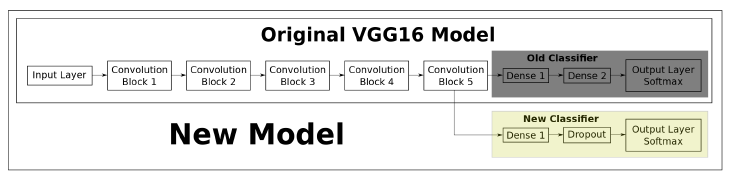
\includegraphics[scale = 0.65]{img/vgg16.PNG}
\caption[Architettura della rete CNN, ottenuta tramite processo di fine-tuning]{Architettura della rete CNN, ottenuta tramite processo di fine-tuning\footnotemark.}
\label{fig-vgg}
\end{figure}



\footnotetext{Source: \url{https://github.com/Hvass-Labs/TensorFlow-Tutorials/blob/master/10_Fine-Tuning.ipynb}}

\vspace{1cm}


Nel 2020, Hizlisoy \textit{et al.}\cite{hizlisoy2021music} hanno studiato come classificare le emozioni indotte dall'ascolto di canzoni tradizionale turche. La rete utilizzata nel processo si basa sulla fusione di due modelli: una CNN, per la ricerca delle feature rilevanti da spettrogrammi di Mel, e una rete LSTM, unita ad una rete neurale profonda, per effettuare la classificazione. Il dataset di musica tradizionale Turca utilizzato è composto da soli 124 frammenti di canzone, dalla durata di 30 secondi l'uno. Le annotazioni sono state effettuate su 3 classi di emozioni, basate su arousal e valence. Le performance ottenute da questo studio sono sorprendenti, raggiungendo un accuratezza massima di 99.19\%. D'altro canto, tale studio rimane limitato ad un piccolo dataset e la musica utilizzata ha il bias di essere selezionata in un dominio molto specifico, peccando quindi in generalizzazione. Tuttavia, lo studio rimane molto interessante, dimostrando come l'unione di diversi modelli di deep learning applicati ad un task di MER possano raggiungere valori di accuratezza molto elevati.



\newpage

\section{Approccio Ibrido}

 Questo approccio, tra i più studiati negli ultimi anni, consente di utilizzare multipli modelli di machine learning, unendo diverse metodologie. Ad esempio, implementando analisi content-based audio e NLP, con l'obiettivo di creare modelli che fanno uso di molteplici tecniche congiunte per riconoscere l'emozione associata ad una canzone. Un primo studio è fornito da Liu \textit{et al. }\cite{liu2020research} con lo sviluppo di un sistema composto da due differenti approcci. Il primo, basato su LSTM, per la parte della classificazione delle feature relative all'audio. Il secondo è ottenuto integrando un sistema chiamato \textit{BERT} (Bidirectional Encoder Representations from Transformers) \cite{devlin2018bert} per la classificazione del testo. BERT è un sistema basato su transformer, sviluppato da \textit{Google AI} nel 2018, capace di raggiungere risultati sorprendenti nei task di NLP. Tale studio dimostra come l'utilizzo di diverse metodologie congiunte consenta di analizzare con maggior precisione l'umore associato alla canzone, cogliendo cosa l'autore volesse comunicare attraverso sia la musica che le parole.  È possibile osservare il modello in questione in figura \ref{fig-liu}. Questa ricerca è stata effettuata utilizzano 1000 canzoni e raggiunge un risultato medio di accuratezza di 79.70\%.

\vspace{2cm}

\begin{figure}[h]
\centering
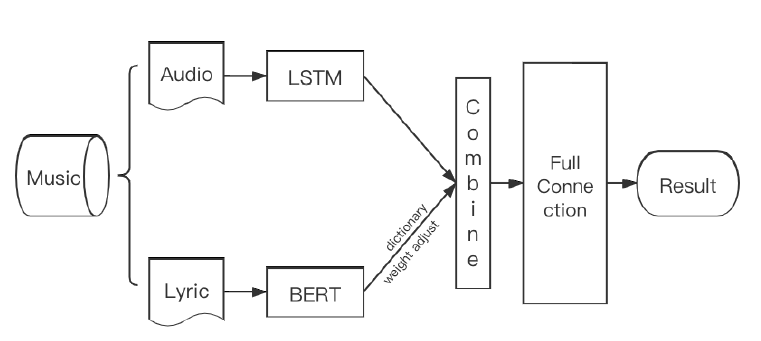
\includegraphics[scale = 0.5]{img/Liu_model.PNG}
\caption{Rappresentazione visiva del modello ibrido utilizzato da Liu \textit{et al.} \cite{liu2020research}.}
\label{fig-liu}
\end{figure}



\chapter{Dataset}

Al fine di ottenere una generalizzazione migliore e non avere problemi di overfitting, causati da un bias dovuto a canzoni troppo simili all'interno di un singolo dataset, sono stati presi in esami 3 diversi dataset utilizzati in ambito MER. Questi dataset sono stati studiati e combinati in modo tale da evitare di avere classi eccessivamente sbilanciate. La scelta delle fonti è stata effettuata utilizzando 3 vincoli sulle proprietà che i dataset dovevano avere:
\begin{enumerate}

    \item I file audio associati alle canzoni dovevano essere disponibili: per poter sfruttare un modello di deep learning capace di analizzare e comprende le emozioni associate ad una canzone era necessario avere a disposizione i file audio da elaborare. Il formato scelto è stato \textit{mp3} essendo quello più comune in questo ambito.
    
    \item Ogni file audio doveva avere una durata di almeno 30 secondi: questo vincolo è stato imposto a causa della necessità di avere una lunghezza fissa per trasformare i file audio in spettrogrammi di Mel, fissata a 30 secondi come descritto nel capitolo successivo.
    
    \item Ogni file audio doveva avere un'annotazione riguardante un'emozione: questo aspetto è fondamentale in uno progetto di deep learning; infatti, ogni campione deve essere propriamente etichettato così da poter addestrare il modello a riconoscere tale etichetta.
    
\end{enumerate}



Una difficoltà riscontrata è stata quella di allineare tutti i vari dataset con un'etichetta basata su uno standard condiviso. Per il progetto è stato scelto di utilizzare 4 etichette, basate sui rispettivi quadranti di Russell. La notazione adottata è visibile in tabella \ref{tab1}. Nella fase di pre-processing tutte le etichette emozionali associate alle canzoni, presenti nei dataset di riferimento, sono state convertite nello standard di annotazione adottato.

\newpage

\begin{table}
\caption{Notazione utilizzata per etichettare le emozioni associate alle canzoni nei quadranti di Russel}
\label{tab1}
\centering
\begin{tabular}{|l|l|l|l|}
\hline
\textbf{Arousal} &  \textbf{Valence} & \textbf{Etichetta} & \textbf{Quadrante}\\
\hline
Basso &  Negativo & 0 & A-V-\\
Basso & Positivo & 1 & A-V+\\
Alto & Negativo & 2 & A+V-\\
Alto & Positivo & 3 & A+V+\\
\hline
\end{tabular}
\end{table}

I tre dataset selezionati ed utilizzati nel progetto sono: \textit{PMEmo}\cite{zhang2018pmemo}, \textit{4Q}\cite{panda2018musical}\cite{panda2018novel} ed \textit{Emotify}\cite{aljanaki2014collecting}\cite{aljanaki2016studying}. 


\section{PMEmo}

\textit{PMEmo}\footnote{https://github.com/HuiZhangDB/PMEmo} è un dataset disponibile pubblicamente alla comunità di ricerca, sviluppato da Zhang \textit{et al}. \cite{zhang2018pmemo} nel 2018. Il dataset è nato per supportare la ricerca, in ambito MER ed affective computing, andando ad annotare le emozioni esplicite ed i segnali fisiologici associati a 457 soggetti in ascolto di musica. Il dataset comprende 794 file audio, corrispondenti ai ritornelli delle canzoni in cima alle classifiche dei brani più ascoltati nel 2016. Nel dettaglio:
\begin{itemize}
    \item 487 canzoni da \textit{Billboard Hot 100};     
    \item 616 canzoni da \textit{iTunes Top 100};
    \item 226 canzoni da \textit{UK Top 40 singles}.
\end{itemize}

I file audio presenti in questo dataset presentano una lunghezza variabile, è stato dunque necessario convertire ogni file ad una lunghezza fissa di 30 secondi. Le annotazioni relative alle emozioni provate dai soggetti in ascolto sono state descritte come un valore compreso tra $[0,1]$ di arousal e valence. Al fine di utilizzare la notazione standardizzata per tutti i dataset è stata effettuata la seguente conversione:

\begin{itemize}
    \item $(Arousal \le 0.5) \wedge (Valence \le 0.5) \to Etichetta = 0$
    \item $(Arousal \le 0.5) \wedge (Valence > 0.5) \to Etichetta = 1$
    \item $(Arousal > 0.5) \wedge (Valence \le 0.5) \to Etichetta = 2$
    \item $(Arousal > 0.5) \wedge (Valence > 0.5) \to Etichetta = 3$
\end{itemize}

Il dataset risulta estremamente sbilanciato, dovuto ad un grande numero di canzoni con annotazione relativa a valence ed arousal maggiore di 0.5, com'è possibile osservare in figura \ref{fig-pmemo}. Per questa ragione, solo un sottoinsieme di 150 file audio è stato utilizzato nell'addestramento del modello finale, con l'obiettivo di evitare un training set troppo sbilanciato.

\begin{figure}
\centering
	\begin{subfigure}[t]{.45\textwidth}
	\centering
    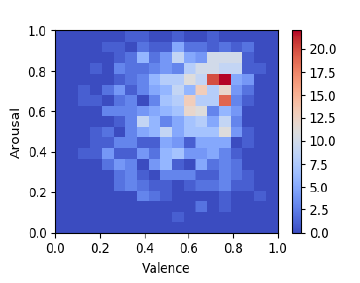
\includegraphics[scale = 0.65]{img/PMEmo_distribution_annotations.PNG}
    \caption{Distribuzione delle annotazioni nel dataset PMEmo \cite{zhang2018pmemo}.}
	\end{subfigure}
	\quad
	\begin{subfigure}[t]{.45\textwidth}
	\centering
    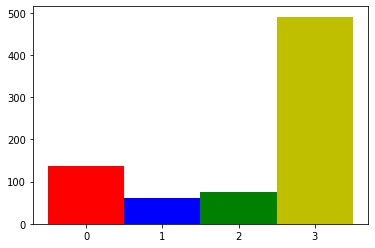
\includegraphics[scale = 0.5]{img/PMEmo-class.png}
    \caption{Distribuzione delle etichette dopo la conversione.}
	\end{subfigure}
	\quad
\caption{Distribuzioni delle annotazioni prima e dopo la conversione.}
\label{fig-pmemo}
\end{figure}


\section{4Q}
\textit{4Q}\footnote{http://mir.dei.uc.pt/downloads.html} è un dataset creato da Panda \textit{et al.} nel 2018 \cite{panda2018musical}\cite{panda2018novel}. Questo dataset contiene 900 file audio musicali suddivise ed organizzate in quattro diverse cartelle, ciascuna contenente 225 file e corrispondente ad un quadrante di Russell. Il dataset contiene inoltre una serie di metadati associati alle canzoni, ad esempio l'artista e il genere di riferimento, tuttavia queste informazioni aggiuntive non sono state tenute in considerazione per il progetto. Le clip musicali sono state ottenute attraverso diverse query all'API \textit{AllMusic}\footnote{http://developer.rovicorp.com} e successivamente sono state filtrate ottenendo un totale di 39983 canzoni. Da questo insieme è stato effettuato un bilanciamento, ottenendo un sotto-insieme di 900 canzoni candidate. Il dataset risultante è estremamente bilanciato e dunque tutte le occorrenze sono state utilizzate ai fini del progetto. Le clip, della durata di 30 secondi, non hanno dovuto subire modifiche e sono state analizzate nella loro interezza.



\section{Emotify}

\textit{Emotify} è un dataset\footnote{http://www2.projects.science.uu.nl/memotion/emotifydata/} creato da Aljanaki \textit{et al.} nel 2014\cite{aljanaki2014collecting}\cite{aljanaki2016studying}. Questo dataset contiene un totale di 400 canzoni, divise per 4 diversi generi: musica classica, elettronica, pop e rock. La musica è stata ottenuta dalla compagnia \textit{Magnatune recording}\footnote{http://magnatune.com/}. Le annotazioni sono state fornite da diversi utenti, tramite un gioco nel quale ogni soggetto poteva ascoltare la traccia audio ed esprimere diverse preferenze, come il gradimento e la scelta di massimo tre emozioni, che descrivessero ciò che ha provato all'ascolto. A differenza dei dataset descritti precedentemente, \textit{Emotify} utilizza delle annotazioni di tipo categorico basate sulla scala GEMS (Geneva Emotional Music Scale) \cite{zentner2008emotions}. Per ciascuna canzone è stata assegnata un'annotazione contente il numero di voti totali per ogni emozione, attribuiti dai partecipanti. È stato quindi necessario, al fine del progetto, scegliere una singola emozione da associare ad ogni canzoni; pertanto, si è deciso di utilizzare la categoria emozionale con il numero di voti più alto. La conversione tra emozioni categoriche nei quattro quadranti di Russell è stata effettuata seguendo lo schema in figura \ref{fig-emotify}.


\begin{figure}
\centering
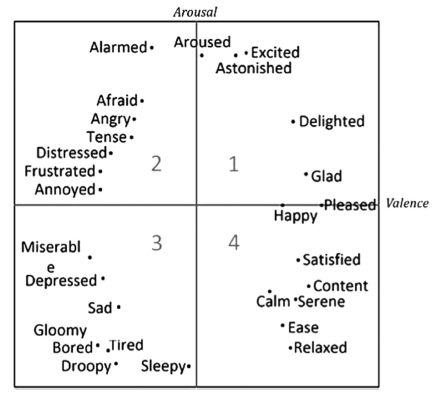
\includegraphics[scale = 0.6]{img/categorical-to-russell.PNG}
\caption{Russell circumplex contenente emozioni categoriche usato per la conversione\cite{panda2018novel}.}
\label{fig-emotify}
\end{figure}


Una volta effettuata la conversione è stato riscontrato che il dataset risultava estremamente sbilanciato, con la maggior parte delle canzoni etichettate come basso arousal e valence positiva: ciò è dovuto probabilmente al numero di aggettivi categorici proposti nel gioco, i quali propendevano per questo specifico quadrante. È possibile osservare lo sbilanciamento citato in figura \ref{fig-emotify2}.
Dunque, anche in questo caso, al fine di evitare un eccessivo sbilanciamento del training set, sono stati utilizzati solamente 150 file audio.


\begin{figure}[h]
\centering
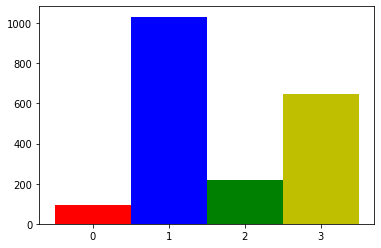
\includegraphics[scale = 0.6]{img/Emotify_class.png}
\caption{ Distribuzione delle etichette dopo la
conversione da categorico ai quadranti di Russell.}
\label{fig-emotify2}
\end{figure}



\newpage

\section{Preprocessing}

Una volta selezionati i dataset da utilizzare è stata effettuata la fase di preprocessing dei dati. In primo luogo, si è standardizzato il sistema di etichettatura utilizzato, come descritto nelle sezioni precedenti, utilizzando metodi di conversioni ad hoc per ogni notazione dei diversi dataset. Una volta che le etichette sono state standardizzate, è stato possibile unire i dataset creando un nuovo insieme contenente 1200 file audio dalla durata di 30 secondi ciascuno. Il modello ideato utilizza una rete CNN per analizzare visivamente le varie canzoni; pertanto, è stato necessario generare per ogni file audio diversi spettrogrammi di Mel. La scelta di utilizzare gli spettrogrammi di Mel è stata fatta sulla base della loro capacità di includere informazioni para-linguali, rendendoli particolarmente utili per task di MER \cite{ma2018emotion}, come dimostrato dallo studio di Bahuleyan \cite{bahuleyan2018music} e Hizlisoy \textit{et al.} \cite{hizlisoy2021music}, descritti nel capitolo 3 relativo allo stato dell'arte. Ogni file audio è stato diviso in 5 frame da 6 secondi, ottenendo 6000 frame, su cui è stato generato lo spettrogramma. Il preprocessing dei file audio e la generazione degli spettrogrammi sono stati implementati utilizzando la libreria Python \textit{Librosa} \cite{mcfee2015librosa}. Un esempio di spettrogrammi di Mel, generati utilizzando la libreria \textit{Librosa}, è possibile vederlo in figura \ref{fig-spectrogram}.\\


I parametri selezionati per la generazione degli spettrogrammi di Mel sono:
\begin{itemize}
    \item \textbf{Frequenza di campionamento:} 22050;
    \item \textbf{Dimensione del frame:} 2048;
    \item \textbf{Hop Size:} 512;
    \item \textbf{Numero di Mel bins:} 96;
    \item \textbf{Dimensione dell'immagine:} 300 x 300 pixel.
\end{itemize}

Infine, il dataset ottenuto è stato diviso in tre sottoinsiemi per effettuare l'addestramento delle reti neurali: training set, test set e validation set. Rispettivamente questi insiemi sono stati ottenuti seguendo la seguente proporzione:
\begin{itemize}
    \item 70\% training set: 4200 frame;
    \item 15\% test set: 900 frame;
    \item 15\% validation set: 900 frame.
\end{itemize}


La divisione è stata effettuata utilizzando gli ID dei file audio, prima della divisione in frame, così da evitare di avere frame relativi ad una stessa canzone in due insiemi diversi. 

\newpage

\begin{figure}
\centering
	\begin{subfigure}[t]{.45\textwidth}
         \centering
         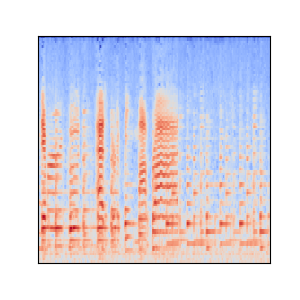
\includegraphics[scale = 0.8]{img/Mel-0.png}
         \caption{Basso Arousal - Valence Negativo}
	\end{subfigure}
	\quad
	\begin{subfigure}[t]{.45\textwidth}
		\centering
        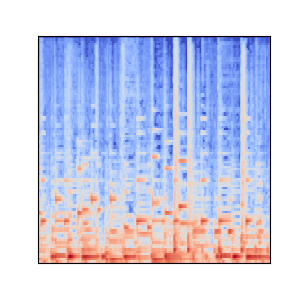
\includegraphics[scale = 0.8]{img/Mel-1.png}
        \caption{Basso Arousal - Valence Positivo}
	\end{subfigure}
	
		\begin{subfigure}[t]{.45\textwidth}
         \centering
         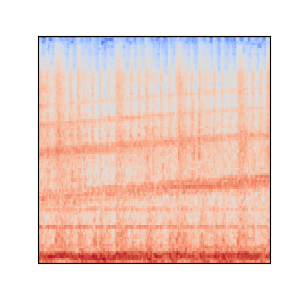
\includegraphics[scale = 0.8]{img/Mel-2.png}
         \caption{Alto Arousal - Valence Negativo}
	\end{subfigure}
	\quad
	\begin{subfigure}[t]{.45\textwidth}
		\centering
        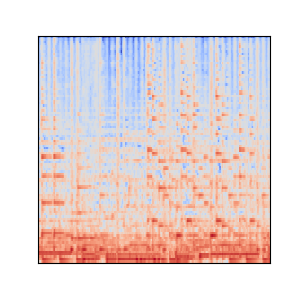
\includegraphics[scale = 0.8]{img/Mel-3.png}
        \caption{Alto Arousal - Valence Positivo}
	\end{subfigure}
	\caption{Esempio di 4 spettrogrammi di Mel generati da file audio etichettati con differenti classi emozionali.}
	\label{fig-spectrogram}
\end{figure}



\chapter{Descrizione dei Modelli MER Proposti}

L'obiettivo del lavoro è quello di creare un sistema di raccomandazione basato su modelli di Deep Learning che sfruttano le emozioni per creare la giusta playlist, in base allo stato emotivo dell'utente. Il modello proposto consiste in due reti fondamentali capaci di ottenere ottime performance in task di riconoscimento emozionale in ambito musicale. Le reti implementate sono:
\begin{itemize}
    \item Convolutional Neural Network (CNN);
    \item Long Short-Term Memory (LSTM).
\end{itemize}

\section{Convolutional Neural Network}

La prima rete impiegata nel modello di riconoscimento emozionale è una 3D CNN. Tale rete è capace di riconoscere i pattern caratteristici e le feature rilevanti degli spettrogrammi di Mel, rispetto alle classi emozionali di appartenenza. La rete è definita 3D perché, oltre a ragionare sulle dimensioni di frequenza e tempo, riesce ad osservare anche il colore dello spettrogramma e quindi a capirne l'ampiezza. Com'è stato possibile notare in figura \ref{fig-spectrogram}, gli spettrogrammi differiscono visivamente quando il mood associato alla canzone è diverso, dunque la rete impara a riconoscere tali differenze.
Al fine di ottenere performance soddisfacenti sono state analizzate due reti neurali convoluzionali pre-addestrate, con performance allo stato dell'arte nel task \textit{ImageNet.} Le reti analizzate presentano sostanziali differenze architetturali, così da scegliere empiricamente quella più adatta ai fini del progetto. Le reti prese in esame sono: \textit{EfficientNet-B3} \cite{tan2019efficientnet} e \textit{MobileNetV3-Large} \cite{howard2019searching}.

\newpage

\subsection{EfficientNet-B3}


Le EfficientNet sono una famiglia di reti neurali convoluzionali, presentate per la prima volta nel maggio 2019 da Tan \textit{et al.} \cite{tan2019efficientnet}, basate su un metodo di model scaling innovativo rispetto ad altre reti allo stato dell'arte. Il vantaggio di questa architettura è la capacità di scalare uniformemente le dimensioni di larghezza, profondità e risoluzione utilizzando un coefficiente composto $\phi$. Nello specifico:
        \begin{equation}
            \begin{split}
                profondità:&\ d = \alpha^\phi\\
                larghezza:&\ w = \beta^\phi\\
                risoluzione:&\  r = \gamma^\phi\\
                s.t.&\ \alpha \cdot \beta^2 \cdot \gamma^2 \approx 2\\
                &\ \alpha\geq1, \beta\geq1, \gamma\geq1
            \end{split}
        \end{equation}
        dove $\alpha$, $\beta$, $\gamma$ sono costanti determinabili da una grid search.\\
        
        La versione B7 di EfficientNet ha raggiunto un'accuratezza top-1, su \textit{ImageNet}, pari al 84.3\%, raggiungendo lo stato dell'arte a parità di \textit{Gpipe} \cite{huang2019gpipe}, pur essendo 8.4 volte più piccola e 6.1 volte più veloce nell'inferenza.
        EfficientNet si è inoltre dimostrata molto performante in caso di utilizzo in transfer learning, in particolare raggiungendo un'accuratezza pari al 91.7\% su Cifar-100 \cite{cifar} e al 98.8\% su Flowers \cite{flowers}.\\
        
        Nel caso dell'obiettivo di riconoscimento emozionale trattato in questo progetto è stata scelta la versione B3, la quale prende in input immagini di dimensione 300x300 pixel. Questa decisione è dettata dal trade-off tra compattezza, quindi limiti hardware, e performance della rete. È possibile osservare l'architettura della rete in figura \ref{fig:efficientnet-arch}.
        Le performance delle varie versioni di EfficientNet su \textit{ImageNet} rispetto ad altre reti sono mostrate in figura \ref{fig:efficientnet}.

\begin{figure}[h]
    \centering
    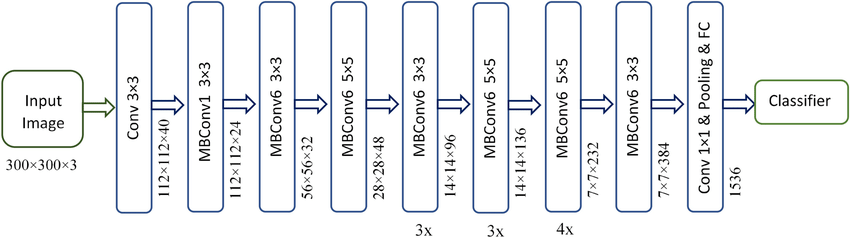
\includegraphics[scale=2]{img/Schematic-representation-of-EfficientNet-B3.png}
    \caption{Architettura compatta della rete EfficientNet-B3 \cite{effnetb3-arch}.}
    \label{fig:efficientnet-arch}
\end{figure}

\newpage


\begin{figure}
    \centering
    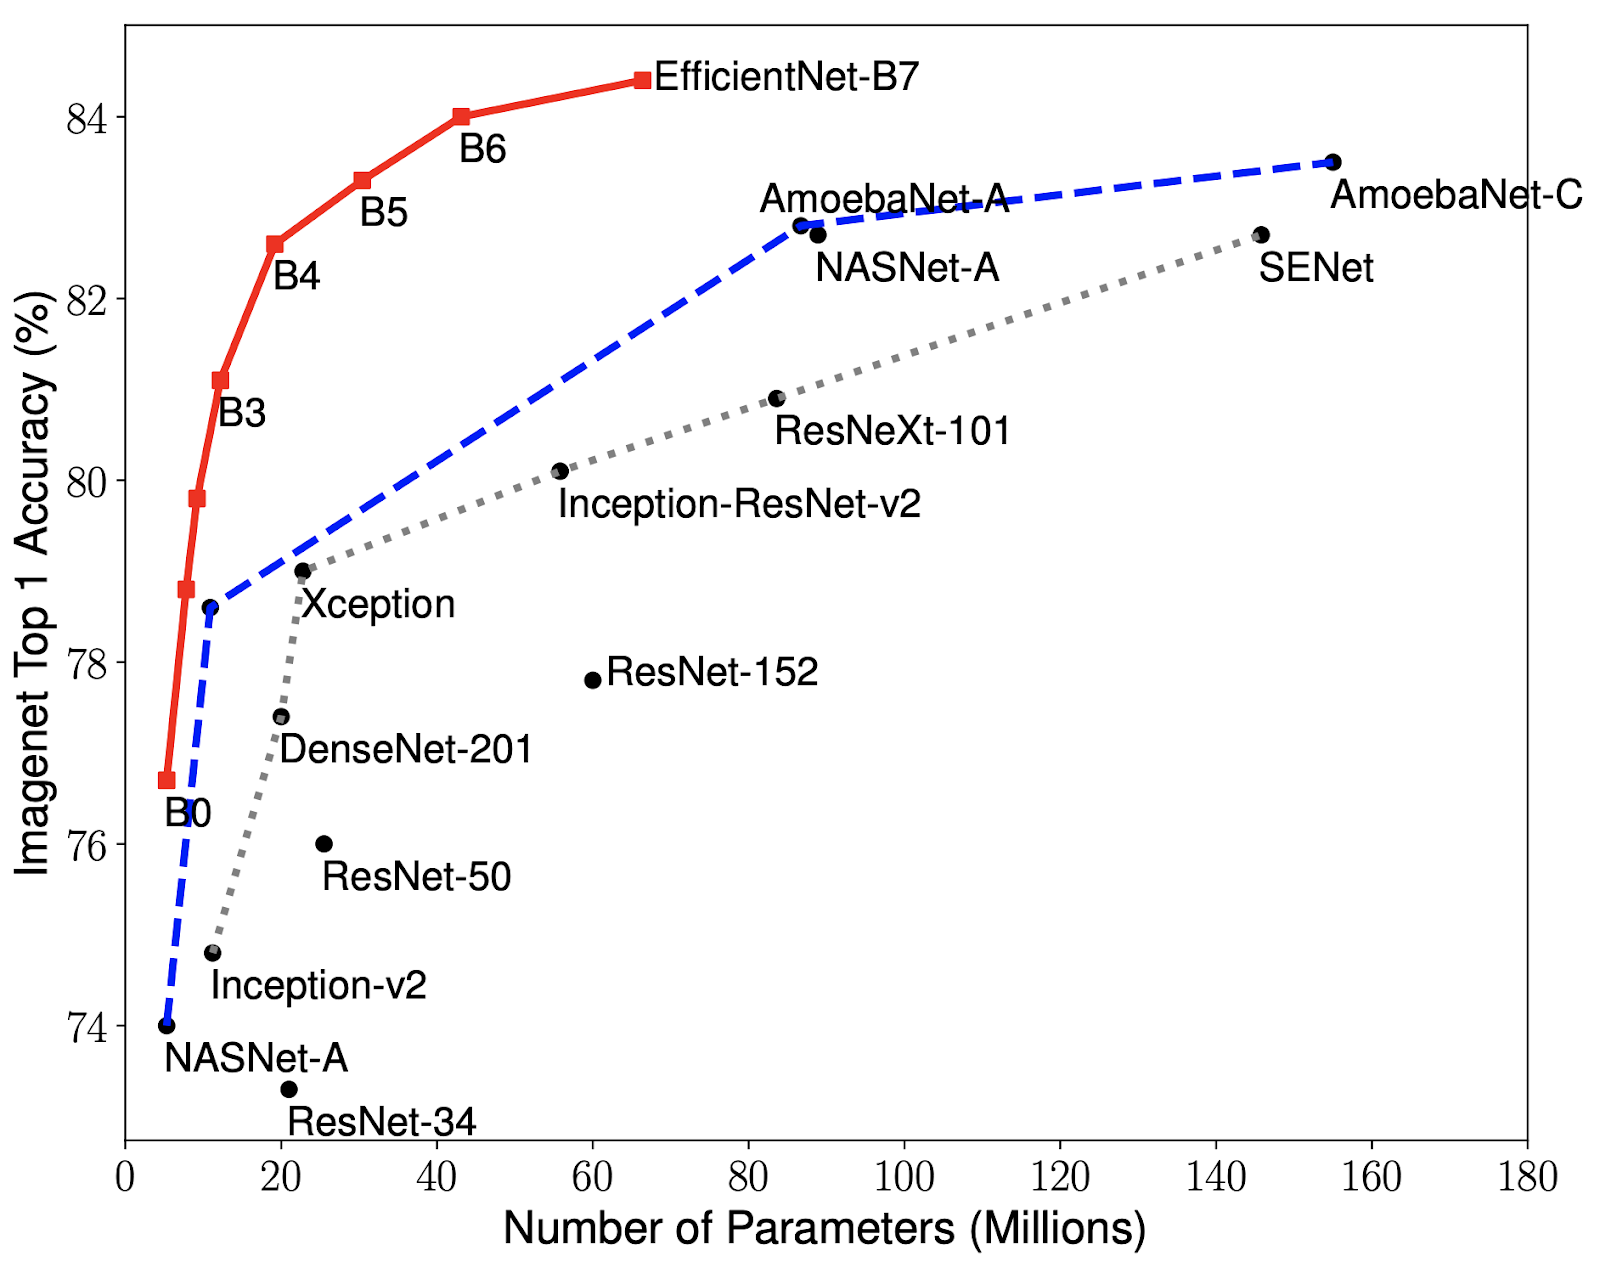
\includegraphics[scale=0.2]{img/efficientnet-performance.png}
    \caption{Performance di EfficientNet rispetto ad altre reti nella challenge \textit{ImageNet}.}
    \label{fig:efficientnet}
\end{figure}


\subsection{MobileNetV3}

La rete MobileNet nasce nel aprile 2017, dallo studio di Howard \textit{et al.} \cite{mobilenet2017} nel creare una rete neurale convoluzionale "leggera", con pochi parametri e basso costo computazionale, così da poter essere utilizzata in applicazioni mobile ed applicazioni embedded di computer vision.  L'architettura utilizza quella che viene chiamata "depthwise separable convolution" (DSC), un metodo che consente di ridurre drasticamente il numero di parametri rispetto ad altre reti con la stessa profondità  \cite{pujara_2020}. Il DSC è formato da due operazioni fondamentali, fattorizzando un layer convoluzionale standard in due layer:
\begin{itemize}
    \item \textbf{Depthwise Convolution}: per ogni canale si effettua una convoluzione spaziale in maniera separata;
    \item \textbf{Pointwise Convolution}: si effettua in coda una convoluzione 1x1 per cambiare la dimensione.
\end{itemize}

L'idea è quella di separare le dimensioni spaziali e la profondità dei filtri, ottenendo reti più profonde ma molto più leggere. È possibile osservare visivamente il DSC in figura \ref{fig:DSC}. I vantaggi principali sono bassa latenza e basso costo computazionale, quindi bassa energia richiesta per l'utilizzo.


\begin{figure}
    \centering
    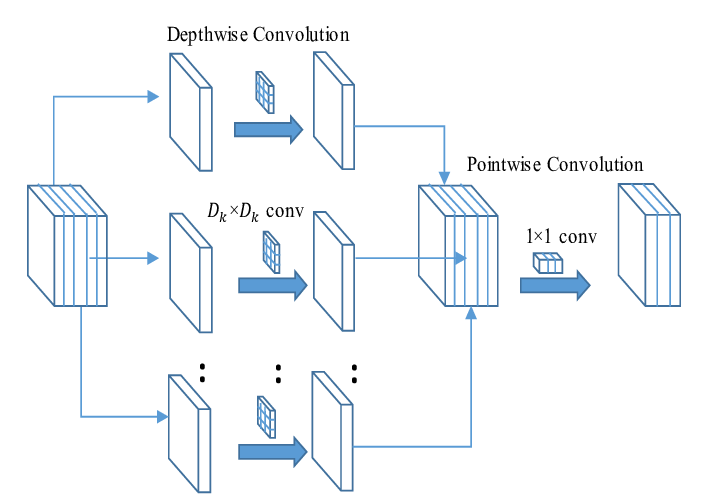
\includegraphics[scale=0.45]{img/Depthwise-separable-convolution-block.png}
    \caption{Depthwise Separable Convolution (DSC) \cite{dsc}.}
    \label{fig:DSC}
\end{figure}


Nel 2019 Howard \textit{et al.} \cite{howard2019searching} rilasciano una versione migliorata dell'originale MobileNet, pubblicando uno studio sulla versione di nuova generazione chiamata MobileNetV3. Tale versione ottiene un miglioramento di circa il 25\% nella velocità di inferenza rispetto alla versione V2, mantenendo la stessa accuratezza. Per ottenere questo avanzamento è stato inserito un layer chiamato "squeeze and excitation". Questo strato, posizionato dietro il global average pooling layer, lavora con feature map molto piccole (1x1) a differenza delle reti precedenti (7x7), alleggerendo la rete \cite{hollemans}. È possibile osservare la comparazione tra la rete originale e la versione V3 in figura \ref{fig:mobv3}. Nel progetto è stata implementata la versione di MobileNetV3 "Large", ovvero quella con più parametri che raggiunge i valori di accuratezza migliore. 

\begin{figure}
    \centering
    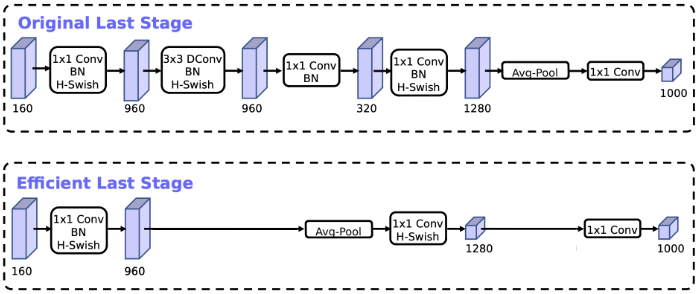
\includegraphics[scale=1]{img/MobileNetV3FinalStage.png}
    \caption{Comparazione tra rete originale e la versione più efficiente V3 \cite{howard2019searching}\cite{hollemans}.}
    \label{fig:mobv3}
\end{figure}

\newpage

\subsection{Addestramento}

Nella fase di training dei modelli sono stati utilizzati in partenza i pesi ottenuti dalle reti su \textit{ImageNet}, al fine di effettuare un transfer learning sul nuovo task di MER. È stato scelto di utilizzare tali pesi grazie alla grande varietà di feature a basso livello riconosciute dalle reti, avendo quindi una buona base di partenza per riconoscere le varie differenze tra gli spettrogrammi. Per effettuare la classificazione sono stati aggiunti all'ultimo layer di output delle CNN i seguenti layer:
\begin{itemize}
    \item Flatten layer: ottiene le feature dall'ultimo layer delle reti CNN e ne cambia forma, togliendo la varie dimensioni agli array e restituendo un vettore ad una dimensione. Questo array monodimensionale sarà l'input della rete fully-connected usata come classificatore;
    
    \item Dense layer di 1024 neuroni: classico strato di una rete fully-connected dove ogni neurone è collegato in input ed output a tutti quelli precedenti e successivi;
    
    \item Dropout Layer con dropout rate di 0.5: strato usato per la regolarizzazione della rete. Ogni iterazione vengono disattivati il 50\% dei neuroni, scelti in maniera causale, così da evitare che l'informazione passi sempre per neuroni troppo specializzati, creando il fenomeno di overfitting. Lo spegnere in maniera random diversi neuroni fa si che l'informazione trovi di volta in volta una via diversa per confluire nella rete, distribuendo meglio i pesi;

    \item Dense layer di 512 neuroni;
    
    \item Dropout layer con dropout rate di 0.4: andando avanti negli strati è bene diminuire la percentuale di dropout dato che i neuroni diventano sempre di numero minore;
    
    \item Dense layer di 128 neuroni;
    
    \item Dropout layer con dropout rate di 0.3;
    
    \item Dense layer di 4 neuroni con funzione di attivazione softmax: layer di output della rete, ogni neurone rappresenta una classe. La funzione softmax ottiene le stime percentuali di appartenenza alle classi e ne sceglie quella maggiore.
\end{itemize}

A tutti i dense layer è stata usata la funzione di attivazione ReLU (Rectified Linear Unit) \cite{relu}, la funzione più utilizzata nelle reti neurali profonde, grazie alla sua capacità di non saturare il gradiente. Inoltre ogni dense layer utilizza anche una regolarizzazione L2 con $\alpha = 0.1$. La regolarizzazione L2, chiamata anche \textit{ridge regression}, viene utilizzata per penalizzare i pesi troppo grossi, evitando quindi fenomeni di overfitting \cite{l1l2}. La funzione obiettivo va a minimizzare la \textit{sparse categorical crossentropy loss}, funzione di errore utilizzata nelle classificazioni multi-classe \cite{loss}.
La funzione di ottimizzazione adottata è stata \textit{Adam} \cite{kingma2014adam} la quale, grazie alle proprietà adattive, riesce a trovare i punti di minimo in maniera estremamente rapida, sfruttando il momentum nella discesa del gradiente. Per stimare il learning rate ottimale è stato utilizzato un algoritmo di ricerca: si effettua un training basato su 5 epoche e si aumenta ad ogni iterazione il learning rate in maniera esponenziale, in un range da 0.0001 ed 1. Il learning rate ottimale risulta quello che consente alla loss di scendere in maniera più ripida. In figura \ref{fig:lr-find} è possibile osservare un esempio del grafico ottenuto dal processo di ricerca descritto. Il training è stato effettuato attraverso 50 epoche, utilizzando un batch size di 32 istanze. Il dataset è stato suddiviso rispettivamente nei sotto-insiemi di training (70\%), validation (15\%) e testing (15\%). Al fine di utilizzare il modello che ha ottenuto performance di generalizzazione migliori, vengono memorizzati solo i pesi che hanno ottenuto i valori di accuratezza maggiori sul validation set. 



\begin{figure}[h]
    \centering
    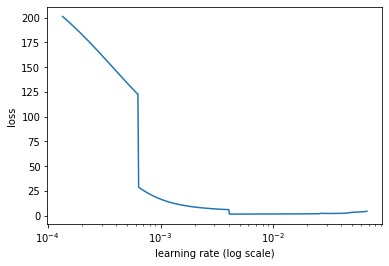
\includegraphics[scale=0.65]{img/lr-finder.png}
    \caption{Grafico raffigurante la curva di loss ottenuta dall'algoritmo di ricerca del learning rate ottimale. Nel esempio specifico il risultato finale è stata del valore di 0.0006.}
    \label{fig:lr-find}
\end{figure}


La libreria utilizzata per implementare il codice \textit{Python} per l'addestramento delle reti è stata \textit{TensorFlow} \cite{tensorflow}, una delle librerie principali relative allo sviluppo di modelli di Deep Learning. I notebook contenenti i training dei modelli sono stati eseguiti sulla piattaforma \textit{Kaggle}\footnote{\url{https://www.kaggle.com/}}, utilizzando le seguenti specifiche hardware:
\begin{itemize}
    \item \textbf{CPU:} Intel(R) Xeon(R) CPU @ 2.30GHz;
    \item \textbf{RAM:} 12GB;
    \item \textbf{GPU:} NVIDIA TESLA P100 16GB.
\end{itemize}



In figura \ref{fig:train-CNN} è possibile osservare le metriche di accuratezza e loss durante la fase di addestramento, relative agli insiemi di training e di validation. Si nota come sia presente overfitting sul training set, pur avendo attuato diversi tipi di regolarizzazioni per evitarlo. Questo è dovuto alla complessità ed al gran numero di parametri delle reti utilizzate. Per far fronte a questo problema si sono utilizzati solo i pesi che hanno ottenuto i migliori punteggi di accuratezza sul validation set, come descritto in precedenza. La metrica di loss invece decresce in maniera netta per entrambi i modelli.



\begin{figure}[h]
\centering
	\begin{subfigure}[t]{.45\textwidth}
	\centering
    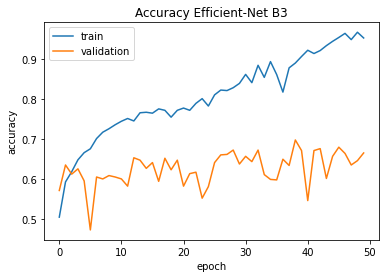
\includegraphics[scale = 0.5]{img/Acc-EffNet.png}
	\end{subfigure}
	\quad
	\begin{subfigure}[t]{.45\textwidth}
	\centering
    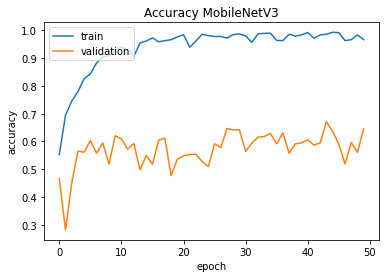
\includegraphics[scale = 0.5]{img/Acc-MobileNet.png}
	\end{subfigure}
	\quad
	\begin{subfigure}[t]{.45\textwidth}
	\centering
    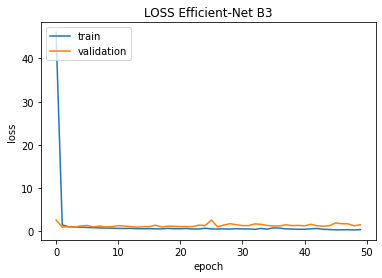
\includegraphics[scale = 0.5]{img/Loss-effnet.png}
	\end{subfigure}
	\quad
	\begin{subfigure}[t]{.45\textwidth}
	\centering
    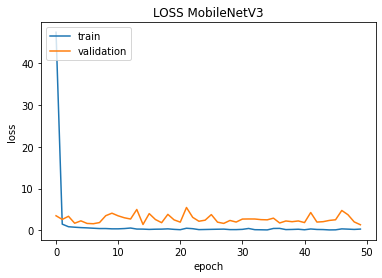
\includegraphics[scale = 0.5]{img/Loss-mobile.png}
	\end{subfigure}
	\quad
\caption{Performance delle reti CNN durante il training.}
\label{fig:train-CNN}
\end{figure}


\subsection{Confronto Risultati}

Le performance ottenute durante l'addestramento non sono sufficienti a valutare il modello. È necessario utilizzare un ulteriore insieme di dati, chiamato test set, per osservare come il modello si comporta su dati che non ha mai visto in precedenza. È importante fare questa ulteriore verifica per avere la certezza che la rete abbia delle buone performance nel mondo reale, ovvero che abbia la giusta capacità di generalizzare. Pertanto, la valutazione dei risultati è stata effettuata sul test set. Le performance sono visibili in tabella \ref{tab2}.

\newpage

\begin{table}[h]
\caption{Performance delle reti CNN.}
\label{tab2}
\centering
\begin{tabular}{|l|c|c|c|c|}
\hline
\textbf{Modello} &  \textbf{Accuratezza} & \textbf{F-score}  & \textbf{Tempo Medio di Training per Epoca}\\
\hline
\textbf{EfficientNet-B3} &  0.69  & 0.67 & 90s\\
\textbf{MobileNetV3} &  0.60 & 0.60 & 32s\\
\hline
\end{tabular}
\end{table}

\vspace{1cm}

Come mostrato in tabella \ref{tab2}, il modello basato sulla rete MobileNet V3 ha un leggero deficit in accuratezza, rispetto la rete EfficientNet-B3. Tuttavia il modello basato su MobileNet ha un tempo medio di training per ogni epoca di quasi un terzo rispetto la controparte. Idealmente, l'applicazione contenente il sistema di raccomandazione, di cui si effettua lo studio, dovrebbe avere la capacità di essere eseguita su dispositivi mobili, quindi con carenza di capacità hardware. Diventa quindi importante considerare l'aspetto relativo alla leggerezza del modello e pertanto la scelta finale cade sulla rete basata su MobileNet, di cui il trade-off tra velocità e performance è risultato favorevole. 




\begin{figure}[h]
    \centering
    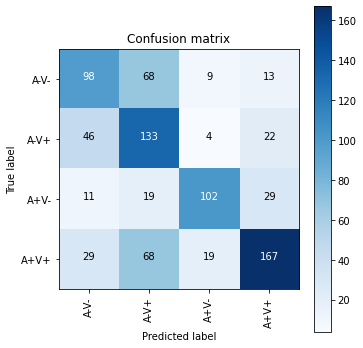
\includegraphics[scale=0.65]{img/CM-MobileNet.png}
    \caption{Grafico raffigurante matrice di confusione ottenuta sul test set dal modello MobileNetV3.}
    \label{fig:cnn-cm}
\end{figure}


Un ulteriore dettaglio relativo all'accuratezza è visibile in figura \ref{fig:cnn-cm} in cui viene mostrata la matrice di confusione relativa a MobileNetV3. Si nota come la diagonale risulta marcata e quindi la maggior parte delle predizioni risulta corretta per ogni classe. Sono visibili alcuni falsi positivi rispetto la classe alto arousal e valence positiva, causati da un leggero sbilanciamento dei dati rispetto a quella specifica etichetta. Nel complesso il risultato è accettabile.




\newpage

\section{Long Short-Term Memory}


La seconda rete impiegata nel modello di riconoscimento emozionale è una LSTM. Una volta che la rete CNN è stata addestrata a riconoscere le feature rilevanti dalle immagini, raffiguranti gli spettrogrammi di Mel, è possibile utilizzarla come feature extractor. La rete LSTM sarà quindi usata come nuovo classificatore del modello finale. Questi modelli sono vastamente utilizzati in task di riconoscimento musicale grazie alla loro capacità di processare informazioni sequenziali \cite{hochreiter1997long}. Al fine di analizzare una porzione di canzone di una lunghezza media, ossia non troppo lunga ma nemmeno eccessivamente frammentata, è stato deciso di utilizzare, come input alla rete, frame audio di 24 secondi. Per ottenere questa lunghezza si generano 4 spettrogrammi, relativi a 6 secondi ciascuno. Quest'ultimi vengono utilizzati come input della rete CNN: le feature estratte in output subiranno un reshape per essere considerate un singolo input, di quattro sequenze, per la rete LSTM. È possibile osservare il processo appena descritto raffigurato in maniera schematica in figura \ref{fig:lstm-feature}.

\vspace{2cm}

\begin{figure}[h]
\centering
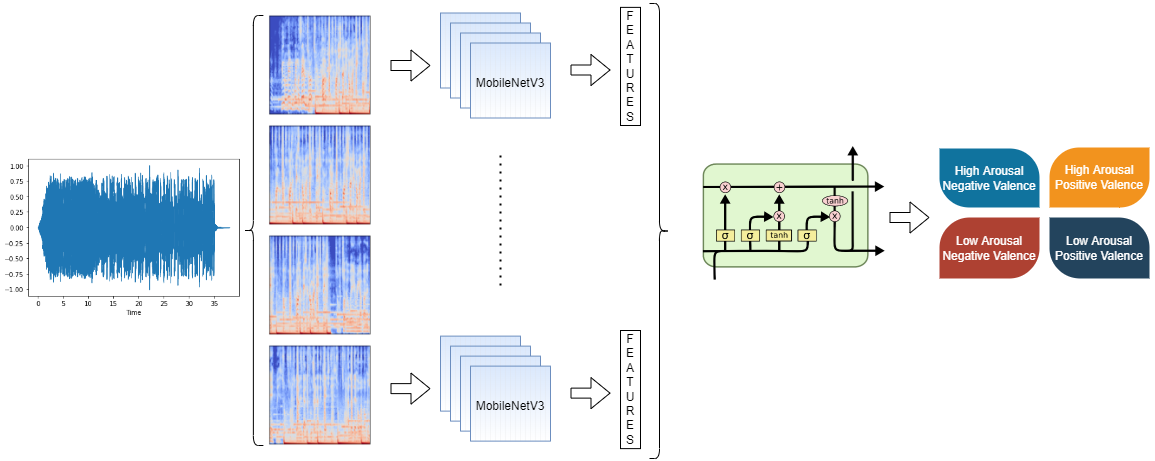
\includegraphics[scale = 0.52]{img/LSTM-Training.png}
\caption{Le feature sono estratte usando la rete CNN ed utilizzate come singolo input di 4 sequenze per la LSTM.}
\label{fig:lstm-feature}
\end{figure}

\newpage


\subsection{Addestramento}

L'architettura della rete LSTM è formata da:
\begin{itemize}
    \item 128 LSTM hidden unit con funzione di attivazione ReLU;
    
    \item Dropout layer con dropout rate di 0.2;
    
    \item Dense layer di 4 output, con funzione di attivazione softmax.
    
\end{itemize}

La funzione obiettivo minimizza la \textit{categorical sparse crossentropy loss}. Viene utilizzata come funzione di ottimizzazione \textit{RMSProp} \cite{tieleman2012rmsprop} poiché presente empiricamente migliori performance quando applicata a reti LSTM. L'addestramento è effettuato utilizzando 20 epoche e una batch size di 32 istanze. Il dataset è stato suddiviso rispettivamente nei sotto-insiemi di training (70\%), validation (15\%) e testing (15\%). Anche in questo caso si andranno ad utilizzare come modello finale i pesi che hanno ottenuto il migliore punteggio di accuratezza sul validation set. Per l'esecuzione del notebook è stato sempre utilizzato \textit{Kaggle}, con le specifiche elencate nello scorso capitolo. È possibile osservare in figura \ref{fig:train-LSTM} le performance ottenute nelle varie epoche, utilizzando le feature ottenute dalla rete MobileNetV3.

\begin{figure}[h]
\centering
	\begin{subfigure}[t]{.45\textwidth}
	\centering
    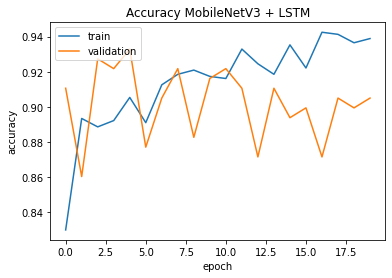
\includegraphics[scale = 0.5]{img/LSTM-accuracy.png}
	\end{subfigure}
	\quad
	\begin{subfigure}[t]{.45\textwidth}
	\centering
    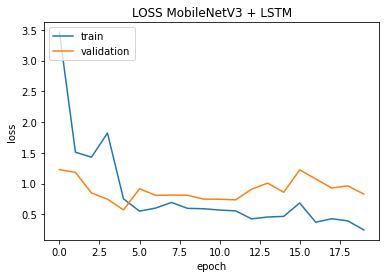
\includegraphics[scale = 0.5]{img/LSTM-Loss.png}
	\end{subfigure}
	\quad
\caption{Performance della rete LSTM durante il training.}
\label{fig:train-LSTM}
\end{figure}


I risultati ottenuti nel training migliorano nettamente i risultati ottenuti tramite l'utilizzo della sola rete CNN. È possibile notare tuttavia un inizio di overfitting, visibile dalla divergenza delle due curve nella crescita di accuratezza. La loss invece decresce e rimane stabile per entrambi i set.

\newpage

\subsection{Risultati}

La rete LSTM raggiunge ottimi risultati anche in fase di testing, raggiungendo uno valore di accuratezza e F-score di 91\%. La matrice di confusione, mostrata in figura \ref{fig:LSTM-cm}, mostra come quasi tutte le classificazioni siano effettuate con successo. I risultati sono in linea con quelli ottenuti dagli studi citati nel capitolo relativo allo stato dell'arte. Il modello dimostra di essere capace di generalizzare in maniera efficace, pertanto risulta utilizzabili ai fini del sistema di raccomandazione.

\vspace{2cm}

\begin{figure}[h]
    \centering
    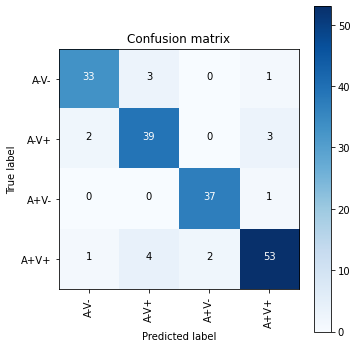
\includegraphics[scale=0.7]{img/confusion-matrix-lstm.png}
    \caption{Grafico raffigurante matrice di confusione ottenuta sul test set dal modello LSTM, basato sulle feature estratte da MobileNetV3.}
    \label{fig:LSTM-cm}
\end{figure}

\newpage

\section{Variazione Intra-Dataset ed Inter-Dataset}

Un aspetto importante da valutare, considerando l'utilizzo di fonti multiple, sono le variazioni dei dati tra i diversi dataset impiegati nel processo di training. Esistono, infatti, dipendenze tra i campioni presenti all'interno di un singolo dataset che possono portare a bias comuni. Ad esempio, le canzoni, selezionate da classifiche di brani più ascoltati in un certo periodo storico, sono soggette alle mode musicali del momento, le quali possono portare ad avere esempi musicalmente simili e quindi ad ottenere dei risultati di performance maggiori che quelle raggiungibili in un'applicazione nel mondo reale, composto da esempi più eterogenei. L'utilizzo di dati da diverse fonti, come nel caso delle tre impiegate in questo lavoro, sono già un espediente per risolvere questo problema di dipendenze tra i dati, fornendo un campione più eterogeneo e quindi aumentando la capacità del modello di generalizzare \cite{intra-inter}. È tuttavia interessante andare a studiare queste dipendenze, effettuando diverse prove empiriche, attraverso l'utilizzo del modello introdotto nei capitoli precedenti. Nello specifico, sono state effettuate 3 diverse prove, con lo scopo di valutare quanto le performance variassero tra modelli addestrati con solo esempi di un dataset, quindi intra-dataset, e modelli addestrati con campioni presi da diverse fonti, quindi inter-dataset.

\subsection{Modello Interamente Addestrato su Singolo Dataset}

Il primo esperimento è stato addestrare il modello finale, composto dalle reti CNN (MobileNetV3) e LSTM, solo su un dataset ed effettuare il test sui rimanenti. Questa prova valuta le performance della rete, addestrata utilizzando solo esempi relativi ad un dataset. Nello specifico è stato selezionato \textit{4Q}, grazie al suo bilanciamento tra classi. Una volta addestrato il modello si verificano le performance, utilizzando esempi ottenuti dalle restanti fonti. Per il testing si è usato l'intero set di dati relativi ai due dataset non utilizzati nel training. Il dataset \textit{4Q} è stato invece diviso nei sotto-insiemi di training (90\%), validation (5\%) e testing (5\%), anche in questo caso ponendo particolare attenzione nel non utilizzare spettrogrammi relativi alla stessa canzone in due insiemi differenti. Così facendo, le feature riconosciute dalla rete CNN appartengono solo a spettrogrammi di un singolo dataset e il classificatore è addestrato a utilizzare solo tali informazioni per effettuare la predizione. I risultati ottenuti, come auspicabile, mostrano un netto distacco tra le performance del modello testato sul dataset di training e quelle relative alle due altre fonti. È possibile osservare le performance ottenute in tabella \ref{tab-es1}. Tale differenza mostra una certa dipendenza tra le canzoni  inter-dataset, tuttavia i valori ottenuti, utilizzando interi dataset come testing, sono accettabili per un problema di classificazione multi-classe e dimostrano che il modello ha una capacità di generalizzazione di circa il 50\%, valore confermato empiricamente nel capitolo 6.

\newpage

\begin{table}[h]
\caption{Riepilogo del modello addestrato sul dataset \textit{4Q} e testato sui restanti.}
\label{tab-es1}
\centering
\begin{tabular}{|c|c|c|c|}
\hline
&\textbf{4Q} &  \textbf{PMEmo} & \textbf{Emotify}\\
\hline
\textbf{Accuratezza} & 0.8  & 0.47 & 0.54\\
\hline
\end{tabular}
\end{table}






\subsection{CNN Addestrata su Singolo Dataset}

Il secondo esperimento va maggiormente nel dettaglio. In questa prova non si addestra l'intero modello su un singolo dataset, ma solo la prima parte della rete, ovvero la CNN. Lo scopo di tale configurazione è quello di andare ad osservare come una rete convoluzionale, addestrata su un solo dataset, riesca ad estrarre feature rilevanti di spettrogrammi generati da altri dataset. Tali informazioni saranno utilizzate per addestrare la rete LSTM. Nello specifico:
\begin{itemize}
    \item Per l'addestramento della rete CNN si utilizza \textit{4Q} suddiviso in training (90\%) e validation (5\%);
    \item Per l'addestramento della rete LSTM verranno utilizzate le feature estratte dall'insieme di training della rete CNN insieme a quelle ottenute dai restanti dataset, sempre suddivisi in training (90\%), validation (5\%);
    \item Per la fase di testing si utilizzano le restanti porzioni dei tre dataset (5\% ciascuno).
\end{itemize}

In questo caso i valori di accuratezza ottenuti, sulle porzioni di test, risultano essere migliorati per entrambi i dataset non impiegati nell'addestramento della rete CNN, ma solo di quella LSTM, in relazione alla prova precedente. È possibile osservare tali valori in tabella \ref{tab-es2}. Questo aumento è imputabile al classificatore, capace di interpretare meglio le feature estratte dalla rete CNN, relative ai dataset non impiegati nell'addestramento di quest'ultima. Un punto a favore di quest'interpretazione è la miglior capacità di classificare esempi relativi alle fonti escluse dal training della CNN. Le performance ottenute sul dataset \textit{4Q} risultano invece leggermente peggiorate: questo è spiegabile a causa di una perdita di specializzazione del classificatore sul dataset di riferimento, in funzione di una migliore generalizzazione.

\vspace{1cm}


\begin{table}[h]
\caption{Riepilogo della modello composto dalla rete CNN, addestrata sul dataset \textit{4Q}, e dalla rete LSTM addestrata su tutti.}
\label{tab-es2}
\centering
\begin{tabular}{|c|c|c|c|}
\hline
&\textbf{4Q} &  \textbf{PMEmo} & \textbf{Emotify}\\
\hline
\textbf{Accuratezza} & 0.75  & 0.59 & 0.65\\
\hline
\end{tabular}
\end{table}


\newpage

\subsection{Modello Addestrato su Insieme Inter-Dataset}

Quest'ultimo esperimento è necessario a verificare come il modello, inteso in tutte le sue parti (CNN e LSTM), si comporti se addestrato sull'insieme congiunto di tutti e tre i dataset. A differenza di quanto visto nel capitolo 5.2, in questa fase non si utilizzeranno dei sotto-insiemi bilanciati dei vari dataset, ma l'intero campione dei dati. Nell'ambito del Deep Learning, l'aspetto più fondamentale per le performance di un modello non è solamente l'architettura della rete, ma soprattutto la qualità dei dati utilizzati in fase di training. L'utilizzo dei dataset completi, senza pre-processing per bilanciare le classi, potrebbe portare a performance peggiori. Anche in questo caso si vanno a creare i tre sotto-insiemi di training (90\%), validation (5\%) e testing (5\%) per ogni dataset e successivamente si uniscono quelli di training e validation per creare un unico grande insieme per l'addestramento della rete. I test invece rimarranno disgiunti, così da poter osservare come un modello inter-dataset si comporti in relazione ai singoli dataset di partenza. In tabella \ref{tab-es3} è possibile osservare i risultati ottenuti.

\vspace{1cm}

\begin{table}[h]
\caption{Riepilogo della modello addestrato tramite l'utilizzo di tutti i dataset, senza bilanciamento delle classi.}
\label{tab-es3}
\centering
\begin{tabular}{|c|c|c|c|}
\hline
&\textbf{4Q} &  \textbf{PMEmo} & \textbf{Emotify}\\
\hline
\textbf{Accuratezza} & 0.73  & 0.77 & 0.57\\
\hline
\end{tabular}
\end{table}

\vspace{1cm}

L'accuratezza ottenuta dai dataset \textit{4Q} e \textit{PMEmo} risulta essere buona, seppur più bassa di quella ottenuta dal modello finale progettato nel capitolo 5.2.  Il dataset \textit{Emotify} invece raggiunge risultati di performance più bassi. Al fine di indagare le ragioni di questa diminuzione di performance generali, sono state generate le matrici di confusione per ogni test set. È possibile osservarle in figura \ref{fig:es3}:
\begin{itemize}
    \item \ref{fig:es3A} (4Q): la matrice di confusione mostra una diagonale marcata, indice di buon bilanciamento nel test set delle classi e di capacità del modello di generalizzare. Si notano tuttavia alcuni falsi positivi relativi alle classi A-V+ e A+V+, ossia le etichette su cui i restanti dataset presentano uno sbilanciamento. Ciò dimostra come la fusione di dataset, con bilanciamenti interni delle classi molto diversi, senza un'opportuna fase di pre-processing, porti ad un peggioramento generale del modello e delle performance ottenute sui dataset con un giusto rapporto tra le classi.
    
    \item \ref{fig:es3B} (PMEmo): questo dataset presenta un estremo sbilanciamento generale dei dati verso la classe A+V+: la maggior parte degli esempi appartengono a questa classe e il modello li riconosce correttamente, a discapito delle restanti etichette. Questo fenomeno è dovuto al partizionamento nei vari insiemi di training e test, i quali mantengono la proporzione sbilanciata del dataset di partenza.
    
    \item \ref{fig:es3C} (Emotify): analogamente a quanto descritto per \textit{PMEmo}, anche in questo caso il dataset presenta un grande sbilanciamento in favore della classe A-V+ e ciò si riflette sulle classificazioni ottenute. Interessante notare come non ci sia nessuna predizione corretta della classe A-V- e A+V-. È possibile notare come molte delle predizioni errate siano falsi negativi della classe maggioritaria, indice di un modello predisposto a generalizzare su un insieme di dati sbilanciato.
\end{itemize}

Al termine di questi esperimenti si ha la prova empirica che la fase di bilanciamento dei dati, attuata durante il pre-processing, sia stata necessaria al fine di addestrare un modello su un insieme bilanciato di dati, migliorando notevolmente le performance. Tuttavia rimane interessante notare come la rete riesca, in alcuni casi, comunque a mantenere performance buone, maggiori del 70\% di accuratezza, anche utilizzando l'insieme sbilanciato dei dataset congiunti. Ciò dimostra che il modello preso in esame sia architetturalmente solido.

\newpage



\begin{figure}[h]
\centering
	\begin{subfigure}[t]{.5\textwidth}
	\centering
    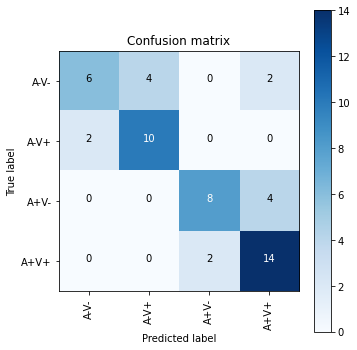
\includegraphics[scale = 0.6]{img/es3-4Q.png}
    \caption{4Q}
    \label{fig:es3A}
	\end{subfigure}
	\quad
	\begin{subfigure}[t]{.5\textwidth}
	\centering
    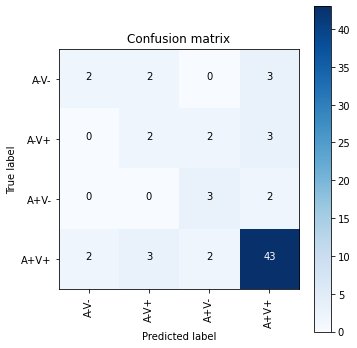
\includegraphics[scale = 0.6]{img/es3-PMEmo.png}
    \caption{PMEmo}
    \label{fig:es3B}
	\end{subfigure}
	\quad
	\begin{subfigure}[t]{.5\textwidth}
	\centering
    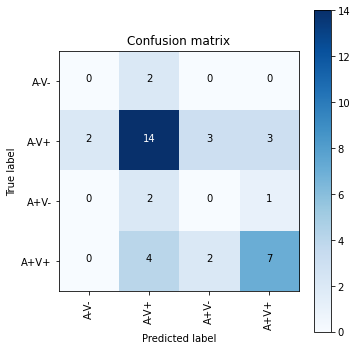
\includegraphics[scale = 0.6]{img/es3-Emotify.png}
    \caption{Emotify}
    \label{fig:es3C}
	\end{subfigure}
	\quad
\caption{Matrici di confusione associate ad ogni test set.}
\label{fig:es3}
\end{figure}

\newpage
\chapter{User-Tuning}


Nello scorso capitolo è stato trattato come si è arrivati ad ottenere un modello di deep learning, in ambito MER, per la classificazione delle emozioni partendo da spettrogrammi di Mel. I risultati ottenuti, sui dataset di partenza, sono stati incoraggianti e le percentuali di accuratezza rilevate dimostrano che il modello riesce a riconoscere correttamente le emozioni. Questa capacità risolve uno dei principali problemi dei sistemi di raccomandazione precedentemente citati, ovvero il cold start. Grazie ad esso si potrà avere una stima, e quindi un'etichetta, subito dopo che una canzone è stata rilasciata, consentendo al sistema di effettuare le raccomandazioni anche senza tag espliciti degli utenti. Inoltre, un utente appena iscritto alla piattaforma potrà usufruire fin da subito delle raccomandazioni per mood, basandosi sul modello generale. Tuttavia le emozioni sono per loro natura soggettive, dunque la rete creata non è capace di riconoscere questa soggettività intrinseca nel problema: risulterà invece ottima nella generalizzazione del task, ovvero nel trovare quale emozioni sia mediamente più probabile rispetto alle altre. Esistono però utenti che hanno percezioni completamente fuori dall'ordinario: ad esempio chi usufruisce unicamente di musica metal è più probabile che tenderà a reputare noiose canzoni commerciali, rispetto a chi invece ascolta quella tipologia di musica. Pertanto il modello generale non è altro che una base di partenza ed è necessario far sì che, per ogni utente, si crei una rete capace di considerare la soggettività dell'individuo, imparando a riconoscere le emozioni nello stesso modo in cui l'utente le percepisce. In deep learning, quando si parte da un modello generale e lo si raffina in uno più specifico, si parla di fine-tuning, tuttavia ai fini del lavoro proposto è stato coniato il termine "\textit{user-tuning}", sottolineando che il processo di fine-tuning è effettuato su ogni singolo utente. L'idea è stata quella di simulare un'applicazione reale, nella quale ogni soggetto può decidere di esprimere in maniera esplicita la sua percezione emotiva, rispetto ad un ascolto. Il modello imparerà dunque a capire il modo in cui l'utente percepisce la musica, basandosi su ognuna delle emozioni da esso indicate. 

\newpage


\section{Modello User-Tuned}


Il modello user-tuned nasce sulla base della rete generale, addestrata nel capitolo precedente: essa sarà il punto di partenza su cui si andrà ad effettuare fine-tuning su ogni utente. Nello specifico, si utilizza la rete CNN MobileNetV3, usata come feature extractor, e la rete LSTM come classificatore. I pesi utilizzati nel modello sono quelli che hanno ottenuto il miglior punteggio di accuratezza nel validation set, ovvero quelli che riescono meglio a generalizzare.

Si può pensare allo user-tuning come un sistema di Federated Learning (FL) \cite{li2020federated}, in cui si passa da una rete unica centralizzata ad un paradigma decentralizzato, dove ogni utente possiede una copia privata del modello, chiamato meta-modello \cite{vanschoren2019meta}, basato su dati di cui esso è proprietario. \\

Per effettuare una prova sperimentale e verificare in maniera empirica se il modello user-tuned riesca davvero ad adattarsi ai singoli utenti, è stato creato un nuovo dataset contenente 50 canzoni, scelte in maniera tale da ricoprire in maniera più organica ed eterogenea possibile i differenti generi musicali. La lunghezza media finale dei file audio è di 280 secondi. I titoli sono stati selezionati tra le canzoni più ascoltate, relative ai diversi generi di riferimento. I generi includono: rock, metal, punk, pop, commerciale, indie, rap, jazz, blues e cantautorato italiano. L'esperimento è stato eseguito su 3 utenti, alla quale è stato richiesto di ascoltare tutte le canzoni ed etichettarle rispetto alla loro emozione predominante all'ascolto. Ogni canzone è stata etichettata utilizzando la notazione valence-arousal descritta nel capitolo 4. Il soggetto poteva inoltre indicare 10 e 20 canzoni di cui voleva che il modello fosse a conoscenza della sua percezione emotiva, così da poter effettuare il fine-tuning.

\subsection{Addestramento}

Partendo dai file musicali, etichettati dall'utente e resi espliciti alla rete, l'addestramento del modello user-tuned è il seguente. Vengono generati gli spettrogrammi di Mel corrispondenti all'intera canzone, suddivisi in frame di 6 secondi ciascuno, ovvero la lunghezza su cui la CNN è stata addestrata ad estrarre le feature rilevanti. Tali immagini sono dunque etichettate con l'emozione suggerita dall'utente e aggiunti al dataset finale ottenuto nel capitolo 4, su cui si è effettuato il training del modello generale. Il modello subirà un processo di fine-tuning con questo nuovo dataset esteso, ricavando le feature dalla CNN ed addestrando il classificatore LSTM sul nuovo insieme di dati, utilizzando un learning rate estremamente piccolo (0.000001) ed attraverso 50 epoche. Il valore del learning rate è stato scelto empiricamente con lo scopo di evitare un eccessivo cambio di pesi durante il training, generando un'eccessiva variazione del modello ed esponendolo ad un overfitting fuori controllo. In questo modo si otterrà un nuovo modello, capace di adattarsi all'utente mantenendo l'abilità di generalizzare. Lo scopo principale di questa fase è quello di generare un overfitting "controllato", così da spingere il modello ad imparare le percezioni dello specifico utente. Al fine di ottenere questo effetto, sono stati utilizzati i nuovi spettrogrammi etichettati, aggiunti al dataset originale anche come validation set, così da poter verificare che il modello abbia imparato correttamente a classificare le canzoni rispetto alla percezione soggettiva dell'utente. Anche in questo caso, il modello finale utilizzerà i pesi che hanno ottenuto il valore di accuratezza migliore sul validation set. Uno schema riassuntivo del processo descritto è visibile in figura \ref{fig:summary-user-tuning}.

\vspace{1cm}

\begin{figure}[h]
\centering
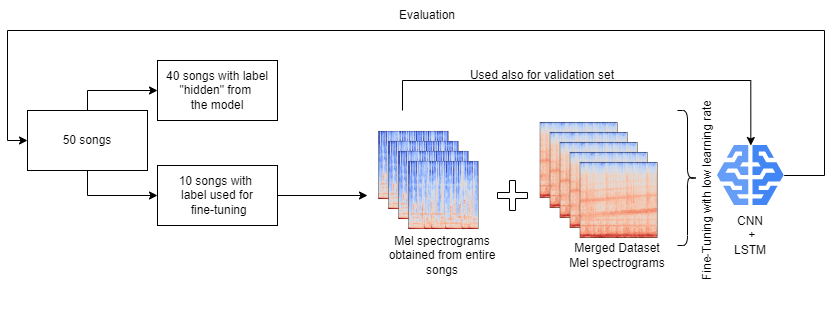
\includegraphics[scale = 0.55]{img/finetuning-process.png}
\caption{Schema riassuntivo del processo di user-tuning.}
\label{fig:summary-user-tuning}
\end{figure}

\vspace{0.5cm}

 Com'è possibile osservare in figura \ref{fig:train-user-tuning}, i risultati ottenuti sono ottimi, sia in termini di accuratezza che di loss. Applicando questa strategia, in fase di training il risultato raggiunto è di un'accuratezza del 89\% sul validation set.

\vspace{0.5cm}

\begin{figure}[h]
\centering
	\begin{subfigure}[t]{.45\textwidth}
	\centering
    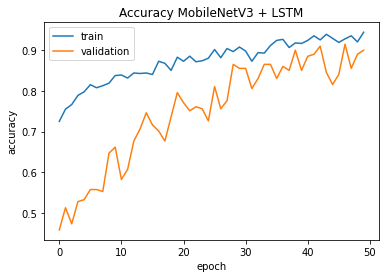
\includegraphics[scale = 0.5]{img/user-tuning-accuracy.png}
	\end{subfigure}
	\quad
	\begin{subfigure}[t]{.45\textwidth}
	\centering
    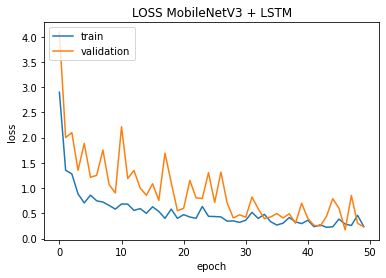
\includegraphics[scale = 0.5]{img/user-tuning-loss.png}
	\end{subfigure}
	\quad
\caption{Performance della rete user-tuned durante il training.}
\label{fig:train-user-tuning}
\end{figure}


\newpage

\subsection{Valutazione dei Risultati}


Il modello proposto in questo lavoro è stato valutato utilizzando il nuovo dataset di 50 canzoni. La valutazione viene effettuata attraverso le informazioni suggerite dai 3 soggetti, impiegati nell'ascolto ed annotazione delle emozioni percepite. Gli esperimenti effettuati per ogni soggetto sono 3:
\begin{itemize}
    \item 0 emozioni suggerite: si utilizzano le 50 annotazioni dell'utente sul modello finale ottenuto senza user-tuning. Risulta importante effettuare questa valutazione al fine di verificare come il modello generale si comporta in una casistica di uso reale;
    
    \item 10 emozioni suggerite: si addestra il modello su solamente 10 delle 50 etichette totali, utile per osservare come il modello si comporta basandosi su pochi suggerimenti dell'utente;
    
    \item 20 emozioni suggerite: si addestra il modello su 20 delle 50 etichette totali. Questo esperimento valuta come il modello si adatti all'utente con un numero modesto di suggerimenti. È atteso un miglioramento all'accuratezza del modello, rispetto alle altre casistiche.
\end{itemize}

Per effettuare questi esperimenti, ogni canzone è stata suddivisa in frame da 24 secondi ed ognuno di essi è stato classificato attraverso la rete LSTM. Ogni frame avrà quindi una predizione del modello: l'etichetta finale trovata, rispetto ad ogni canzone, sarà data dalla predizione che otterrà maggior frequenza rispetto alle 4 classi emozionali. Così facendo, per ogni canzone si otterrà non solo una singola stima emozionale, ma una lista con le percentuali di frequenza rispetto a tutte le classi, come mostrato in figura \ref{fig:prediction-user-tuning}. Questo risulta molto utile per fare distinzioni tra due canzoni che hanno una stessa classe emozionale: alcune avranno una percentuale più alta dell'etichetta finale rispetto ad altre, potendo quindi fare ulteriori distinzioni al momento della raccomandazione. Questo argomento verrà trattato in maniera più estesa nella sezione successiva, relativa al sistema di raccomandazione e generazione playlist proposto.

\begin{figure}[h]
\centering
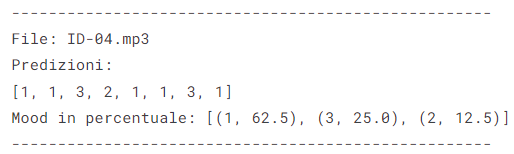
\includegraphics[scale = 0.9]{img/user-tuning-prediction.PNG}
\caption{Esempio di output del modello relativo al file con ID = 04. Vengono mostrate le predizioni relative ai frame di 24 secondi ed infine la stima percentuale per ogni classe emozionale.}
\label{fig:prediction-user-tuning}
\end{figure}


\newpage

\begin{figure}
\centering
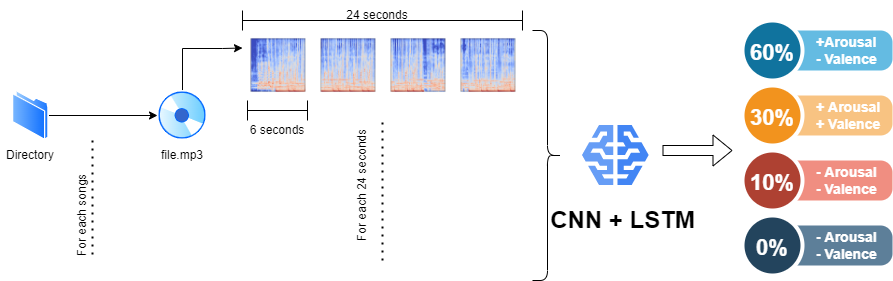
\includegraphics[scale = 0.5]{img/evaluation.png}
\caption{Diagramma dell'algoritmo di classificazione del modello user-tuned, applicato all'intero dataset di canzoni.}
\label{fig-user-evaluation}
\end{figure}

\vspace{1cm}

Dopo aver compilato un file \textit{csv} per ogni esperimento svolto, annotando tutte le etichette trovate dai soggetti, è stato creato uno script Python che, preso in input la cartella contenente le 50 canzoni ed il file \textit{csv}, esegue i seguenti step:

\begin{enumerate}
    \item Per ogni file audio nella directory genera dei spettrogrammi di Mel, relativi alla durata di 6 secondi ciascuno;
    
    \item Le feature rilevanti sono estratte dalla rete CNN MobileNetV3 considerando 4 spettrogrammi ad ogni iterazione, relativi a 24 secondi totali;
    
    \item Le feature ottenute dai 4 spettrogrammi subiscono una trasformazione in un singolo vettore, contenente i 4 vettori di feature: questo passaggio è necessario per essere considerati un singolo input di 4 sequenze per la rete LSTM;
    
    \item  La rete LSTM genera diverse predizioni, una per ogni sequenza della lunghezza di 24 secondi;
    
    \item Una stima percentuale di tutte le predizioni effettuate, rispetto ad una canzone, viene memorizzata. Tale stima mostra i vari mood che cambiano all'interno di una canzone. Il mood che ottiene la percentuale maggiore verrà selezionato come classe finale. Nel caso una canzone abbia due valori con la stessa stima percentuale come maggioritari ne verrà selezionato solo uno.
    
    
\end{enumerate}

Un diagramma dell'algoritmo descritto è visibile in figura \ref{fig-user-evaluation}.


\newpage

Al fine di valutare le performance del modello user-tuned non basta utilizzare semplicemente l'accuratezza, basata sulla stima dell'emozione più frequente. È stato ritenuto opportuno introdurre una nuova metrica di errore, per quantificare la distanza tra la stima ottenuta come risultato della classificazione e l'emozione reale annotata dal soggetto, nel caso le due etichette divergano. Questa metrica stabilisce quanto il modello si è sbagliato nell'effettuare la predizione: un valore alto significa che la stima dell'emozione annotata dall'utente è stata nulla, ovvero non è stata mai rilevata nella canzone. D'altro canto un valore basso, ad esempio minore di 25, significa che, anche se l'emozione non è stata trovata correttamente, il modello non ha sbagliato di molto. Tale stima è quindi calcolata come la differenza tra la frequenza dell'emozione predetta (quella che ha ottenuto il valore maggiore) e la frequenza della vera classe emozionale del soggetto. Una volta ottenute tutte le stime di errore è stato possibile calcolare l'errore medio totale del modello. È stata utilizzata la seguente formula:
\begin{equation}
\begin{multlined}
\forall_i: \text{ wrong emotion}_i > \text{true emotion}_i: \\
\frac{1}{n  = \text{Number Wrong Predictions}} \sum_{i}^n \text{wrong emotion}_i - \text{true emotion}_i
\end{multlined}
\end{equation}


Un errore medio alto significa che il modello non sta performando bene, inoltre grazie a questa metrica è possibile valutare come la rete si comporta aumentando il numero di canzoni suggerite nel processo di user tuning. La figura \ref{fig-output} mostra un esempio di output, relativo a 5 canzoni (righe nella tabella) del classificatore user-tuned, in termini di frequenza di ogni classe emozionale, la corrispondente classe predetta dal classificatore (colonna Max\_Overall\_Emotion), comparata alla vera etichetta (User\_Emotion) ed in fine la metrica di errore proposta (Difference).



\begin{figure}
\centering
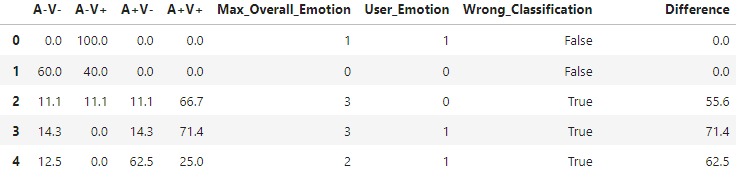
\includegraphics[scale = 0.62]{img/example-output.PNG}
\caption{Esempio del risultato ottenuto su 5 canzoni dopo l'esecuzione del modello. Le prime 4 colonne corrispondono alle stime percentuali dei quadranti di Russell. La colonna \textit{Max\_Overall\_Emotion} corrisponde alla classe emozionale con la frequenza rilevata più elevata. La \textit{User\_Emotion} rappresenta l'etichetta annotata dal soggetto. Nel caso le due colonne non contengano lo stesso valore l'errore (\textit{Difference}) è calcolato.}
\label{fig-output}
\end{figure}

\newpage


Il risultato medio, ottenuto sulle 50 canzoni, per ogni utente e configurazione, è riportato rispettivamente nelle tabelle \ref{tab3} e \ref{tab4}. I risultati mostrano diversi aspetti importanti da considerare:
\begin{itemize}
    \item Per quanto riguarda il modello generale, ovvero quello non soggetto ad user-tuning, è possibile osservare che la media di accuratezza è del 45\%. Tale valore, contestualizzato in un task di classificazione multi-classe ed in contesto reale risulta più che accettabile. 
    
    \item In riferimento ai modelli soggetti ad user-tuning, i risultati sono ottimi. Come atteso, le canzoni suggerite al modello risultano sempre corrette nella classificazione. L'accuratezza, mostrata nei grafici \ref{fig-data1} e \ref{fig-data2}, ottiene un netto miglioramento all'aumentare delle canzoni suggerite. Ciò dimostra che il sistema proposto di user-tuning, valutato in un contesto reale, comporta un'esperienza utente migliore, basata su un modello che impara a riconoscere le percezioni soggettive, in un costante processo di miglioramento tramite l'utilizzo del sistema. Un altro aspetto fondamentale da tenere in considerazione è la metrica di differenza errore proposta: è chiaramente visibile in figura \ref{fig-data2} come questa subisca una decrescita costante all'aumentare delle canzoni suggerite. Questo fenomeno è spiegabile come un sostanziale miglioramento nel modello, non solo sulle canzoni suggerite, che quindi impara in maniera diretta a classificare correttamente, ma anche su quelle che non vengono classificate correttamente. La rete, infatti, imparando le percezioni dell'utente, riesce a classificare in maniera sempre migliore anche le canzoni che non sono suggerite al modello. Questo addestramento passivo è molto importante perché consente di classificare correttamente anche nuove canzoni mai viste dal modello, senza che l'utente debba per forza indicare direttamente l'emozione provata all'ascolto.
\end{itemize}

A fronte di questi valori è possibile affermare che i risultati ottenuti risultino promettenti, tuttavia è necessario estendere lo studio ad ulteriori soggetti, al fine di determinare se, con un bacino di utenza più ampio ed eterogeneo, le performance mantengano questo livello di precisione.


\newpage



\begin{figure}[h]
\centering
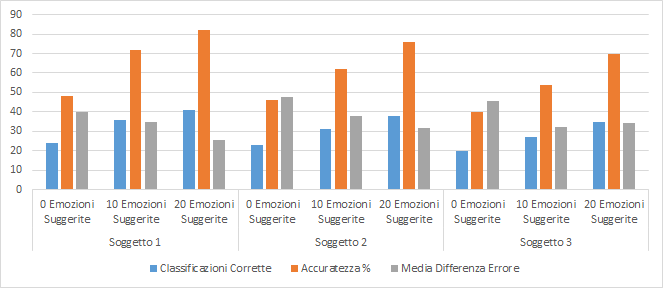
\includegraphics[scale = 0.85]{img/grafico-tab3.png}
\caption{Grafico risultati ottenuti basati sui tre soggetti.}
\label{fig-data1}
\end{figure}

\vspace{2cm}

\begin{figure}[h]
\centering
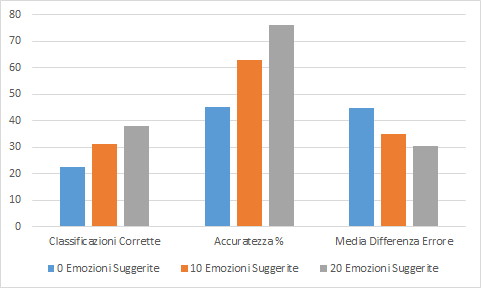
\includegraphics[scale = 0.9]{img/grafico-tab4.png}
\caption{Grafico risultati medi ottenuti per configurazione.}
\label{fig-data2}
\end{figure}



\newpage

\begin{sidewaystable}[ph!]
\thisfloatpagestyle{empty}
\caption{Valutazione basata sui tre soggetti.}
\label{tab3}
\begin{tabular}{|c|c|c|c|c|}
\hline
 \textbf{Soggetto} & \textbf{User-Tuning} &  \textbf{Classificazioni Corrette} & \textbf{Accuratezza \%}  & \textbf{Media Differenza Errore}\\
\hline
&0 Emozioni Suggerite &  24  & 0.48 & 40.03\\
 \textbf{1}&10 Emozioni Suggerite &  36   & 0.72 & 34.92 \\
&20 Emozioni Suggerite &  41   & 0.82 & 25.29\\
\hline
&0 Emozioni Suggerite &  23  & 0.46 & 47.73\\
 \textbf{2}&10 Emozioni Suggerite &  31  & 0.62 & 37.88\\
&20 Emozioni Suggerite &  38  & 0.76 & 31.80\\
\hline
&0 Emozioni Suggerite &  20  & 0.40 & 45.83\\
 \textbf{3}&10 Emozioni Suggerite &  27  & 0.54 & 32.20\\
&20 Emozioni Suggerite &  35  & 0.70 & 34.43\\

\hline
\end{tabular}

\vspace{1cm}

\caption{Valori medi per ogni configurazione.}
\label{tab4}

\begin{tabular}{|c|c|c|c|}
\hline
\textbf{User-Tuning} &  \textbf{Classificazioni Corrette} & \textbf{Accuratezza \%}  & \textbf{Media Differenza Errore}\\
\hline
\textbf{0 Emozioni Suggerite} &  22.34  & 0.45 & 44.62\\
\hline
\textbf{10 Emozioni Suggerite} &  31.33  & 0.63 & 35\\
\hline
\textbf{20 Emozioni Suggerite} &  38  & 0.76 & 30.51\\
\hline
\hline
\end{tabular}
\end{sidewaystable}



\chapter{Sistema di Raccomandazione}

L'ultimo tassello mancante, del sistema proposto in questo lavoro, è quello riguardante l'impiego del modello creato, ovvero il sistema di raccomandazione con cui l'utente si interfaccerà. Come descritto nel capitolo relativo allo stato dell'arte dei sistemi di raccomandazione musicale, la tipologia di modello adottata è quella utilizzata nei sistemi model-based: l'architettura è basata su un modello di deep learning che effettua classificazioni basate sullo specifico utente. Le feature utilizzate entrano nella tassonomia dei sistemi content-based audio analysis, ovvero quelli che utilizzano informazioni direttamente ricavate dai file audio per effettuare le predizioni. Il progetto, tuttavia, non ha l'obiettivo di creare un sistema di raccomandazione classico in ambito musicale, in cui l'utente può filtrare tra le sue canzoni per trovare quelle con il mood richiesto, ma fa un passo ulteriore. È stato posto il focus su un sistema che potesse generare vere e proprie playlist basate sul mood di riferimento dell'utente. 


\section{Generatore di Playlist}


Nell'ambito dei sistemi di raccomandazione musicali, i generatori automatici di playlist possono essere considerati una loro sotto-categoria specializzata. Per generare una playlist è necessario sfruttare un sistema di raccomandazione al fine di creare un elenco nelle corde dell'utente, che contenga ciò che esso ha voglia di ascoltare in quel momento. Una playlist non è altro che una lista di riproduzione musicale, dove i titoli generalmente appartengono ad un insieme logico scelto dall'utente. Ad esempio, esistono playlist basate sui generi musicali, sul mood delle canzoni, sulla data d'uscita dell'album di riferimento, sull'evento dove dovrà essere riprodotta e tanti altri. Nel caso relativo al progetto, la playlist da generare sarà basata sul mood delle canzoni, rilevato dal modello user-tuned. L'idea principale è stata quella di simulare un'applicazione reale, integrata in un'app mobile di riproduzione audio, oppure in una delle piattaforme di streaming musicale presenti sul mercato, dove un utente può dichiarare il proprio umore di partenza e quello che vorrebbe raggiungere alla fine dell'ascolto. Il sistema genererà una playlist che avrà nelle canzoni al suo interno una graduale variazione nell'emozione suscitata nell'utente, così da consentirgli di raggiungere lo stato emotivo atteso. Un'illustrazione è mostrata in figura \ref{fig:playlist-emozioni}.



\begin{figure}[h]
\centering
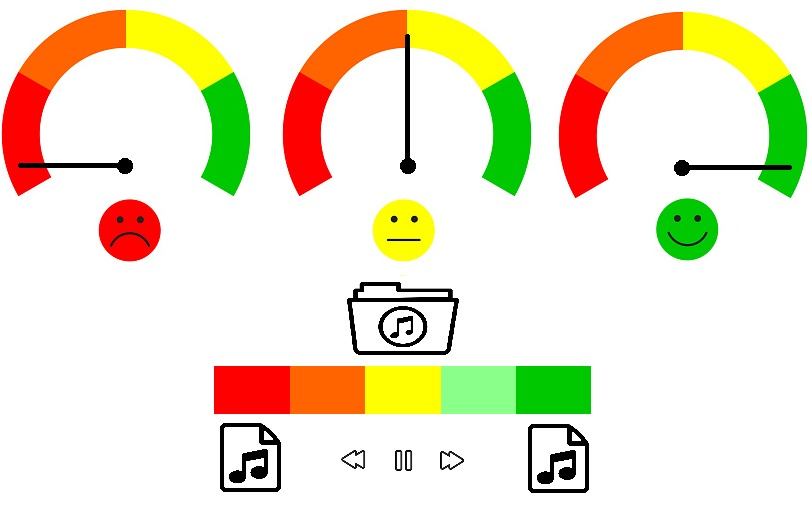
\includegraphics[scale = 1.5]{img/playlist-emotion.jpg}
\caption{Illustrazione relativa al funzionamento della playlist generata. La playlist è strutturata per variare l'umore dell'utente durante l'ascolto in maniera graduale.}
\label{fig:playlist-emozioni}
\end{figure}


\section{Integrazione Modello User-Tuned}

Come descritto nel capitolo precedente, lo scopo finale di questo lavoro non è solo il dimostrare la fattibilità nel creare un modello di Deep Learning capace di riconoscere il mood delle canzoni ed adattarsi alla percezione dell'utente. L'obiettivo è infatti quello di rendere usabile tale modello in un contesto reale di utilizzo, da parte di diversi utenti. L'output generato dalla rete è stato studiato fin dal principio per essere usabile da un sistema di raccomandazione: invece di generare un unica classificazione per ogni canzone, si effettua anche una stima percentuale dei mood contenuti al suo interno, come è stato possibile osservare nella figura \ref{fig-output} della sezione precedente. L'utente finale potrà quindi selezionare il suo umore di partenza e quello che vorrà raggiungere alla fine dell'ascolto della playlist e, tramite una variazione delle percentuali emozionali contenute in ogni canzone, tale passaggio di mood sarà reso guidato e mai repentino. La playlist generata partirà la riproduzione dalle canzoni che hanno una percentuale emozionale, che corrisponde a quella dell'utente, con valori elevati e mano a mano scenderà di percentuale lasciando spazio a quella desiderata. Questo passaggio risulta importante per non creare nell'utente un salto di umore troppo drastico: ad esempio, se esso si trova in uno stato emotivo triste (basso arousal e valence negativa) e vuole raggiungere un mood felice (alto arousal e valence positiva), l'iniziare a riprodurre canzoni classificate come il target richiesto fin dall'inizio potrebbe infastidire e far terminare l'ascolto.

\section{Algoritmo Progettato}

Ai fini di implementare ciò che è descritto nella sezione precedente è stato sviluppato il seguente algoritmo:
\begin{enumerate}

    \item Si richiede all'utente di definire il mood attuale e quello target. Inoltre viene richiesto il numero di canzoni della quale dovrà essere composta la playlist (\textit{playlist\_length}).

    \item Si verifica che il mood di partenza e quello target non coincidano: nel caso siano uguali la playlist sarà generata usando canzoni con valore percentuale elevato dell'emozione selezionata;
    
    \item Si inizializzano le variabili \textit{starting\_value} ed \textit{target\_value} rispettivamente a 100 e 0. Queste variabili rappresentano la stima percentuale dell'emozione di partenza dell'utente (\textit{starting\_value} = 100) e quella target da raggiungere (\textit{target\_value} = 0).
    
    \item Si definisce la variabile \textit{jump}, ovvero quanto dovrà aumentare la percentuale del mood target ad ogni iterazione e quanto dovrà diminuire quella attuale. La funzione per trovare il valore ottimale è definita come:
    
    \begin{equation}
jump = \frac{100}{playlist\_length - 1}
    \end{equation}
    
    
    
    \item Si definisce la funzione \textit{find\_nearest}: dato in input il dataframe contenente tutte le predizioni del modello, il valore percentuale del mood di partenza e il valore percentuale target, essa restituisce l'elemento che ha la distanza tra i due valori di input minore. Ad esempio, se in input si passano i valori di partenza = 70 e target = 30, la funzione restituisce l'elemento che ha le percentuali più vicine a i valori passati (es. partenza = 75, target = 25) tra tutti gli elementi del dataframe delle predizioni. 
    
    \item Si itera sulla \textit{playlist\_length} e, a ogni iterazione, viene trovata la canzone con la minor distanza dai valori di riferimento tramite la funzione \textit{find\_nearest}, aumentando la percentuale target e diminuendo quello iniziale di \textit{jump}. Un esempio di output ottenuto in questa fase è visibile in figura \ref{fig:playlist1}.
    
    \item Si riproduce la playlist ottenuta, come in figura \ref{fig:playlist2}.
\end{enumerate}

L'algoritmo, scritto in Python, nella sua interezza è visibile in appendice A.

\newpage

\begin{figure}[h]
\centering
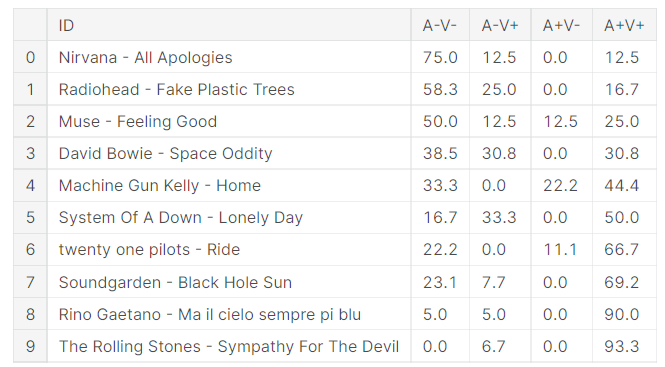
\includegraphics[scale = 0.95]{img/output-playlist.PNG}
\caption{Esempio di output ottenuto con parametri \textit{starting\_mood} = A-V-, \textit{target\_mood} = A+V+ e \textit{playlist\_length} = 10.}
\label{fig:playlist1}
\end{figure}

\vspace{2cm}

\begin{figure}[h]
\centering
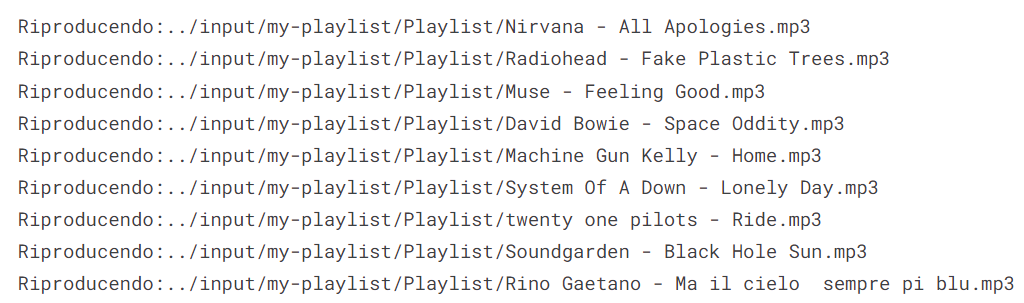
\includegraphics[scale = 0.8]{img/output-playlist-play.PNG}
\caption{Esempio di output finale dello script, i file audio corrispondenti alle canzoni vengono riprodotti.}
\label{fig:playlist2}
\end{figure}




















\chapter{Conclusione}

In questa tesi è stato presentato un nuovo approccio, basato sulle emozioni, per i sistemi di raccomandazione e generazione di playlist. L'applicazione della tecnica MER permette di riconoscere le emozioni, indotte dalle canzoni, al fine di creare diverse playlist personalizzate sulla base dello stato emozionale dell'utente che usufruisce del sistema. Tale metodologia consente di accentuare il focus sul singolo soggetto, migliorando l'esperienza di utilizzo e risolvendo uno dei problemi principali dei sistemi di raccomandazione: il "cold start". 

Nella prima parte è stata esplorata la letteratura di riferimento delle diverse tipologie di sistemi di raccomandazione, in ambito di Music Emotion Recognition, e lo stato dell'arte delle possibili metodologie applicabili. Successivamente sono stati descritti i dataset utilizzati, andando a definire per ognuno di essi le caratteristiche specifiche e le operazioni di pre-processing necessarie all'utilizzo. Infine sono stati esposti i dettagli tecnici di progettazione. 


Il sistema ottenuto al termine della progettazione è basato su due diversi modelli: uno generale e uno "user-tuned". Quello generale è stato progettato impiegando diverse reti neurali: CNN, per l'estrazione di feature rilevanti da spettrogrammi di Mel associati alle canzoni, e LSTM come classificatore delle sequenze ottenute. Il sistema risultante, addestrato sull'unione bilanciata di diversi dataset presenti in letteratura, ha ottenuto ottimi risultati in fase di training, dimostrando la possibilità, da parte di nuovi utenti, di utilizzarlo fin dal primo accesso all'applicazione. Un altro vantaggio importante nell'impiego di questo modello è la capacità di applicarlo non solo a nuovi utenti, ma anche a canzoni mai etichettate prima, osservando la risoluzione di ciò che è definito cold start. Il modello "user-tuned", ottenuto tramite tecnica di fine-tuning applicata a quello generale, consente di imparare direttamente dall'utente il suo modo di percepire emozionalmente la musica, basandosi su alcuni suggerimenti diretti ed adattandosi, migliorando notevolmente l'esperienza. I risultati empirici, ottenuti tramite prove sperimentali applicate a tre soggetti, hanno dimostrato che il modello "user-tuned" riesce a perfezionare le inferenze delle canzoni non suggerite direttamente al sistema, abbassando l'errore di predizione. Infine, la generazione della playlist proposta utilizza le informazioni ricavate dal modello per garantire un passaggio dall'umore attuale dell'utente a quello desiderato in maniera graduale, utilizzando le canzoni dell'utente etichettate dal sistema ed evitando cambiamenti troppo repentini che potrebbero rovinare l'esperienza di ascolto. A fronte dei risultati ottenuti è possibile immaginare l'integrazione del sistema proposto in piattaforme di streaming o applicazioni di riproduzione musicale, le quali difficilmente tengono conto della dimensione emozionale dell'utente.



\section{Sviluppi Futuri}

Esistono diversi possibili sviluppi futuri applicabili al progetto di tesi:

\begin{itemize}
    \item I risultati ottenuti, per quanto promettenti, risultano limitati ad un piccolo bacino di utenti. Effettuare nuovi test, basati su un campione di utenza più ampio, è un passo necessario al confermare le potenzialità, e trovare eventuali limiti, del sistema proposto.
    
    \item Le architetture delle reti neurali utilizzate nella creazione del sistema possono essere ulteriormente migliorate, facendo uso di nuove tecnologie che stanno prendendo sempre più piede in ricerca chiamate \textit{transformer}. Tali modelli, applicati inizialmente a task di NLP, si stanno dimostrando sempre più robusti in applicazioni di pattern analysis, andando a superare le performance di reti CNN \cite{transformer}. Sebbene le reti convoluzionali hanno al momento una letteratura di riferimento più ampia e consolidata, i transformer stanno avendo molto risalto ed è possibile che in un futuro prossimo soppianteranno completamente le prime.
    
    
    \item I dataset utilizzati presentavano alcuni difetti nel bilanciamento dei dati, rendendo necessario una fase di pre-processing per ridurre il problema. Un possibile sviluppo futuro è dato dall'ampliamento di questi dataset con ulteriori esempi, al fine di utilizzare una maggiore mole di dati in fase di addestramento, migliorando la capacità del modello di generalizzare. Un'ulteriore possibilità è quella di applicare strumenti di domain adaptation basati su istanze, come Kliep \cite{kliep} e TrAdaBoost \cite{tradaboost}. Tali tecniche consentono di bilanciare diverse fonti di dati, andando a cambiare il peso di ogni istanza in base alla sua fonte di appartenenza, come mostrato in figura \ref{fig-instance}.
    
    
    \begin{figure}[h]
\centering
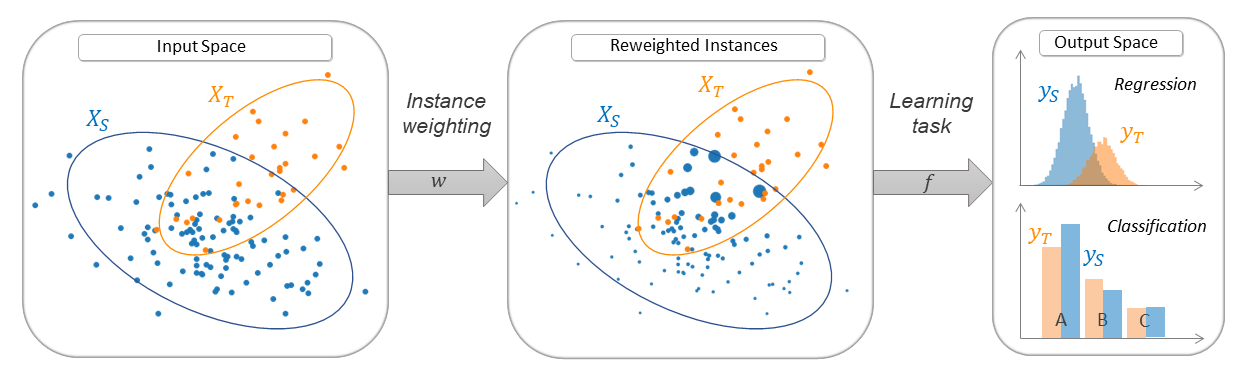
\includegraphics[scale = 0.44]{img/instance_based.png}
\caption[Funzionamento di metodi domain adaptation basati su istanze.]{Funzionamento di metodi domain adaptation basati su istanze\footnotemark.}
\label{fig-instance}
\end{figure}

\footnotetext{Source: \url{https://adapt-python.github.io/adapt/contents.html#adapt-instance-based}}


\item Infine, una possibile estensione del progetto è quella di utilizzare segnali ottenuti tramite sensori indossabili, ad esempio braccialetti per il riconoscimento dello stato emozionale in tempo reale, entrando nel campo del Wearable Computing. Gli studi presenti in letteratura riguardanti l'utilizzo di segnali fisiologici ottenuti direttamente da dispositivi indossabili hanno mostrato ottimi risultati empirici, con percentuali di accuratezza nella stima dell'emozione dell'utente elevate. Ad esempio Ayata \textit{et al.} \cite{wearable} hanno proposto un sistema di classificazione delle emozioni attraverso un modello che utilizza segnali fisiologici multi-canale basati su \textit{galvanic skin response} (GSR) e \textit{photo-plethysmography} (PPG) per inferire l'emozione nello spazio continuo arousal-valence. Questo studio utilizza tali segnali per integrare un sistema di raccomandazione esistente, estendendone le capacità e migliorando le raccomandazioni. L'utilizzo di uno strumento simile nel progetto consentirebbe di rimuovere il bisogno di richiedere esplicitamente all'utente l'emozione attuale, in fase di generazione della playlist, riconoscendola automaticamente. Ciò porterebbe anche ad avere una maggior quantità di dati per effettuare un addestramento più accurato per la fase di user-tuning del modello.

\end{itemize}



\newpage

\appendix
\chapter{Codice Python Generazione Playlist}
%Python code highlighting
\begin{lstlisting}[language=Python, caption=Playlist-Generator.py]
# dati relativi alla creazione playlist, personalizzabili
playlist_length = 10
starting_mood = 'A-V-'
expected_mood = 'A-V-'

# funzione che prende in input le colonne relative alla stima del mood e il valore atteso a cui esse devono avvicinarsi
def find_nearest(array_starting, value_starting, array_target, value_target):
    
    # gli array contengono la differenza tra il valore reale e quello atteso
    starting = np.abs(array_starting - value_starting)
    target = np.abs(array_target - value_target)
    
    # si sommano i valori degli array
    nearest_array = starting + target
    
    # l'elemento minore sara quello con i due mood combinati che piu si avvicinano all obiettivo
    return nearest_array.argmin()

# si inizializza la lista di riproduzione vuota 
song_list = []


if starting_mood != expected_mood: 
    # caso nel quale l'utente vuole shiftare mood
    jump = (100/(playlist_length-1))
    starting_value = 100
    expected_value = 0




    # si itera sulla lunghezza della plylist
    for i in range(playlist_length):

        # viene trovato l'indice della canzone da aggiungere
        idx = find_nearest(df[starting_mood].to_numpy(), starting_value, df[expected_mood].to_numpy(), expected_value)
        
        # alla playlist viene aggiunta la canzone
        song_list.append(df.iloc[idx]['ID'])
        
        # si cancella la canzone aggiunta dal dataframe per evitare di aggiungerla due volte alla playlist
        df = df.drop(idx)
        
        # l'indice del dataframe viene resettato
        df = df.reset_index(drop=True)
        
        # i valori di partenza e target vengono aggiornati in base al valore del salto
        starting_value = starting_value - jump
        expected_value = expected_value + jump
        
else: # il mood dell'utente non deve cambiare, si la playlist cerca tutte le canzoni con il mood richiesto massimizzato
    df = df.sort_values(by=[starting_mood])
    df = df[len(df)-playlist_length:]
    song_list = df['ID'].to_numpy()
\end{lstlisting}


\addcontentsline{toc}{section}{Bibliografia}
\bibliographystyle{IEEEtran}
\bibliography{bibliografia.bib}


\end{document}
